\documentclass[12pt,twoside, parskip=half, headsepline=on, chapterprefix=true, draft=off]{scrbook}

\usepackage[english]{babel}
\usepackage[T1]{fontenc}
\usepackage[utf8]{inputenc}
\usepackage{lmodern}
\usepackage{graphicx}
\usepackage{amsmath}
\usepackage{caption}
\usepackage{color}
\usepackage{adjustbox}
\usepackage[breakable,skins]{tcolorbox}

\renewcaptionname{english}{\chaptername}{Module}

\definecolor{shadecolor}{gray}{0.5}

%\usepackage{hyperref}
%\hypersetup{colorlinks=true, urlcolor=[rgb]{0.25,0.41,0.88}, linkcolor=[rgb]{0.25,0.41,0.88}, pdftitle=Course, pdfauthor=Niko, pdfsubject=, pdfkeywords=}
\usepackage{scrlayer-scrpage}

\ihead{CECAD -- IIAM} 
\chead{} 
\ohead[]{\headmark} 
\renewcommand*{\chapterpagestyle}{scrheadings}
\pagestyle{scrheadings}

\newcounter{taskcounter}
\newenvironment{taskbox}[1]{%
	\begin{tcolorbox}[enhanced,breakable,colframe=red!75!black]%
	\begin{addmargin*}[1em]{1em}%
			\refstepcounter{taskcounter}%
			\vspace{0.5cm}\textbf{Exercise} \textbf{\thechapter.\arabic{taskcounter}:} #1%
			\\\rule[0.9em]{\linewidth}{1pt}%
}{%
	\end{addmargin*}%
	\end{tcolorbox}%
}

\usepackage{natbib}


%% Start Document

\begin{document}

% title 
\title{An Introduction to Image Analysis in Microscopy}
\subtitle{CECAD Imaging Facility Course, v1.1} 
\author{Nikolay Kladt}
\date{\today}
\publishers{Imaging Facility\\Cluster of Excellence -- Cellular Stress Responses in Aging-Associated Diseases\\University of Cologne}

\maketitle


\tableofcontents

% Module 1: Publishing microscopy data (The Basics)
\chapter{Publishing microscopy data}

In this module, we will work through some necessary basics of image processing and explore common ways to visualize microscopy data. After this module, you should feel comfortable working with your images in Fiji and be able to use this knowledge to prepare your data for publication.

Digital images are ubiquitous and nearly everybody is used to taking pictures with a digital camera or smart-phone and also storing and processing these images. The same way that digital imaging has replaced analog cameras in our daily lives, light microscopes have transformed to digital imaging systems\footnote{In this course, we do not discuss the technologies that actually generate digital images in microscopes. If you want to learn about various microscopy techniques, we recommend looking at the online iBiology Microscopy Course (www.ibiology.org/ibioeducation/taking-courses/ibiology-microscopy-course.html, 25-02-2015)}. Even the most simple light microscopes are usually equipped with a digital camera and a screen to display, take and store images - also allowing quick and simple image processing tasks without the need for additional software (e.g. brightness \& contrast adjustments, white balancing). More complex light microscopes, such as confocal laser scanning microscopes (CLSM), already require sophisticated software interfaces to set up imaging parameters and visualize the results. Finally, there are also types of microscopes that depend on digital image processing (e.g. stochastic optical reconstruction microscope, STORM or single plane illumination microscopy, SPIM).

As a result of these advancements, modern digital microscopy offers more than just 'pretty pictures' - there are many imaging techniques that rely on computational analysis as well as methods for image enhancement, restoration and quantitative analysis. Modern microscopy cannot be understood without the basics of digital images and digital image processing. This knowledge is not only essential to make full use of the capabilities, but also to understand limitations -- a very important prerequisite to maintain scientific validity.

\minisec{Raster and vector images}
Typically, most pictures you work with (scanned documents, photos taken with a digital camera, pictures found on the web) are raster graphics (see Fig. \ref{fig:bitmap-graphics}). This means that these images are made up of a grid of \emph{pixels} (picture elements). Each pixel has a value that represents some property of the image (usually brightness). The range of this value is called \emph{bit-depth} and determines possible values at each pixel. Sometimes, the term \emph{bitmap image} is used for a raster image. For example, the image shown in figure \ref{fig:bitmap-graphics} illustrates a raster image with 420 x 420 pixels and a bit-depth of 1 byte. Therefore, we have a total of 176400 pixels, multiplied with 1 byte taking up a total of 172 kilobytes disc space. As you can see, the number of pixels and the bit-depth affect the required disc space. Additionally, we cannot easily change the size of the image; enlarging causes the image to look 'pixelated' or we have to use interpolation techniques to estimate the value of added pixels. Decreasing the number of pixels in the image might result in a loss of image features. There are plenty of commercial and open-source programs to work with raster images; representative software packages are Adobe Photoshop (Adobe Inc., San Jose) and GIMP (GNU Image Manipulation Program, The GIMP team, http://gimp.org).

\begin{figure}[!ht]
	\centering
		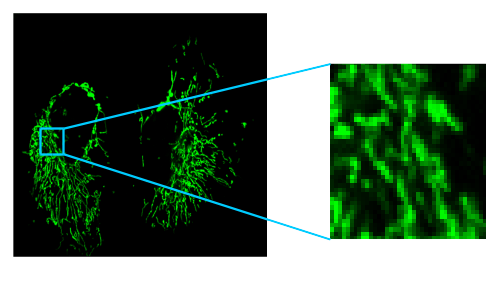
\includegraphics[width=0.60\textwidth]{mod1/figures/bitmap-graphics.png}
	\caption{Fluorescent labeled mitochondria in HeLa cells. THis image shows that raster graphics are made up of pixels that become clearly visible when zoomed.}
	\label{fig:bitmap-graphics}
\end{figure}


In contrast, vector graphics are not made up of a bitmap. Instead, they are based on geometrical shapes such as lines, curves, polygons or other shapes that are based on mathematical expressions. Therefore, these images can be scaled without a loss in image quality and typically use less disc space than raster images. Especially when the scaling of lines, text or other image content might change, it makes sense to use vector graphics (e.g. figures for a manuscript, scientific poster). Similar to the editors for raster images, there are plenty of vector graphics programs; representative examples are Adobe Illustrator (Adobe Inc., San Jose) and Inkscape (The Inkscape team, http://www.inkscape.org).

Often, programs support the conversion between raster and vector graphics. These are called \emph{rasterization} and \emph{vectorization}. Usually, vector graphics programs allow you to include raster-graphics without conversion.

Let's say you're done for the day and want to submit another great manuscript to Nature (Nature Publishing Group). Nature has detailed requirements on how your figures should be prepared for print (http://www.nature.com/nature/authors/gta/3c\_Final\_artwork.pdf, as of 08.10.2014). According to their guide, they prefer vector graphics for text and line-art. We will revisit the Nature figure requirements as we go along discussing properties of digital images!

\begin{verse}
\emph{Can you explain why journals prefer vector graphics for text and line-art?}
\end{verse}

\section{Pixels, spatial resolution and sampling frequency}
\label{sec:mod1-samplingrate}

It is important to remember that our microscopes have an optical resolution\footnote{For this course, we assume that you have a basic understanding why microscopes have an optical resolution and on which parameters the optical resolution depends.} that defines the ability to resolve details of the specimen. 

Limited by the optical resolution, the number of discrete pixels in a digital image then determines the spatial resolution. The number of pixels is usually called the sampling frequency (or sampling interval). This simply means that the spatial resolution depends on the number of pixels within given physical dimensions and that the maximum spatial resolution is limited by the optical resolution\footnote{This is only partially true -- we can theoretically build a microscope where the detector is the limiting factor. In general, the detector is chosen to match the optical resolution; and all internal microscope components involved in generating the digital image have to be matched as well.}. It is important to note that each pixel represents the average response of the optical system measured at a point within an area that is specified by the characteristics of our optical system. 

In a typical confocal microscope (not camera based), we can choose the number of pixels with which we want to sample the acquired image. A change in the pixel number obviously changes the size of the pixel and therefore also the area of which the average response is obtained. Choosing the wrong sampling frequency is a typical pitfall in microscopy, especially when zoom controls are used. If we sample inadequately, details can be lost. Oversampling is usually not critical, we just increase the amount of data we have to handle and we have to know that we oversample. Fortunately, sampling theory tells us exactly which sampling interval (pixel size, pixel number) is required to optimally represent the biological specimen given our optical resolution (the famous \emph{Nyquist theorem} states that we require a sampling interval $\geq$ twice the highest spatial frequency in our specimen and the highest frequencies we can observe are physically limited by our optical resolution). 

This raises the question why our microscopes even allow us to change the sampling frequency and not always simply operate at the diffraction-limited configuration. The reason is, that there are many experimental situations where it is desirable to intentionally lower our spatial resolution. Basically, we have to make a trade-off between the required resolution and imaging speed, amount of light collected at each pixel, photo-toxicity or other experimental parameters. The important thing is that we are aware of the fact that we under-sample for whatever reasons we have.

The limited number of discrete pixels in an image acquired with a microscope has serious consequences when you create figures for a manuscript. Publishers often require a certain number of pixels per cm (inch) to create high-quality figures and unfortunately, they leave it up to you to adjust your figures. However, they usually ignore the fact that you only have a limited number of pixels in your original data. One option you have is resampling your original data to change the number of pixels. Another option is to show pixels enlarged -- leading to a pixelated view of your data.

\subsection{Resampling Images}

Resampling an image changes the original data; the number of pixels is either increased or decreased (enlarging, shrinking). In comparison, using the zoom tool (icon magnifying glass) just increases or decreases the size of the pixels on your screen without resampling. Similar to other programs, Fiji also allows you to change the size of the canvas (the space on which your image is drawn, see Figure \ref{fig:adjust-canvas-dialog}. If you adjust the canvas size \texttt{[Image > Adjust > Canvas Size]}, the image is either cut (pixels outside the canvas size are cut off) or a margin is added where added pixels usually have the background color (zero value). 

\begin{figure}[!ht]
	\captionsetup{justification=centering}
	\centering
		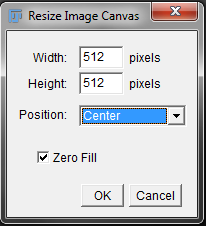
\includegraphics{mod1/figures/adjust-canvas-dialog.png}
		\caption{Adjust Canvas Size Dialog.}\label{fig:adjust-canvas-dialog}
\end{figure}

As you saw above, we determine the number of pixels during image acquisition according to our needs and the limits of the microscope. However, when you prepare your data for a presentation, poster or manuscript you will usually have to scale your original data. Before we discuss best practices and look at an example, we will introduce important basic terminology.

\minisec{Image resolution outside microscopy}

In printed images and in document scanners, resolution is often given in \emph{DPI (Dots Per Inch)}, the number of dots within a line that spans 1 inch (2.54 cm). Computer screen, tablet or phone resolution is typically given in \emph{PPI (Pixels Per Inch)}, the number of pixels within a line that spans 1 inch. Confusing, DPI is often used when PPI would be better, and even more confusing, one printer dot is usually not equal to one pixel! 

As we learned in section \ref{sec:mod1-samplingrate}, knowing the number of pixels is not sufficient to define the resolution -- pixel size (sampling rate, distance of pixels, ..) is necessary as well. This is also true for consumer products such as digital cameras, smartphones or flatscreen TVs. Knowing that a Full HD TV is capable of displaying 1920 x 1080 pixels presents no information about the size of each pixel. An 18 mega-pixel camera that is able to generate photos with 5184 x 3456 pixels also has no resolution associated. For screens, we can calculate the PPI by dividing the number of pixels by the size of the screen. For example, a 40'' Full HD TV would have 55.07 PPI, an IPhone 5 about 326 PPI (4'', 1640 x 1136 pixels but two dots per pixel!), an Amazon Kindle Paperwhite 212 PPI (6'', 1024 x 758). 

High quality photo printing requires about 200-300 PPI. With the number of pixels of our digital camera, we can calculate the maximum size of a high-quality print. For example, an 18 mega-pixel camera print with at least 200 PPI: 

\begin{quotation}
	18 mega-pixel = 5184 x 3456 pixels, divided by 200 PPI results in a print of about 65 x 43 cm (1 inch = 2.54 cm).
\end{quotation}

Publishers usually require that you submit your figures in 300-600 DPI (meaning PPI), depending on the content (e.g. see the requirements of Nature\footnote{http://www.nature.com/nature/authors/gta/3c\_Final\_artwork.pdf, as of 08.10.2014} or PNAS\footnote{http://www.pnas.org/site/misc/digitalart.pdf, as of 04/03/2015}). This already determines the maximum size of your (sub)figure given available pixels. 

\begin{taskbox}{Resampling Example - No Interpolation}

\begin{enumerate}
	\item Open the file resampling-test.tiff in /module1/data. This is a 20x20 pixel black-and-white (binary) image. Use the magnification tool to zoom to the maximum magnification. You should now see a one pixel wide and a two pixel wide vertical white line and a 1px diagonal line. 
	\item Before we perform image manipulations, we duplicate the original image for convenience \texttt{[Image > Duplicate]}.
	\item Go to [Image > Adjust > Size], you should see a dialog as shown in figure \ref{fig:adjust-size-dialog}.
	
	\begin{minipage}[t]{\linewidth}
		\begin{center}
		\adjustbox{valign=t}{%
			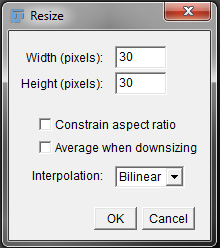
\includegraphics[width=0.3\textwidth]{mod1/figures/adjust-size-dialog.png}%
		}
		\medskip
		\captionof{figure}{Adjust Size Dialog.}\label{fig:adjust-size-dialog}
		\end{center}
	\end{minipage}
	
	\item Perform a resize to 30 x 30 pixels (150\% size), with no interpolation, and compare the result with the original figure. Use the \texttt{Line-Tool} (see fig. \ref{fig:line-tool}) to measure the width of both vertical lines. You should observe that one line was not scaled while the other was scaled to 150\%.
	
	\begin{minipage}[t]{\linewidth}
		\begin{center}
		\adjustbox{valign=t}{%
			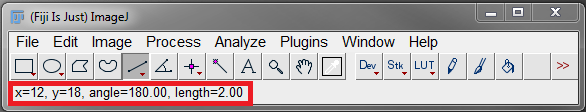
\includegraphics[width=0.7\textwidth]{mod1/figures/line-tool.png}%
		}
		\medskip
		\captionof{figure}{Line tool selection and values.}\label{fig:line-tool}
		\end{center}
	\end{minipage}
	
	\item Try other values for the resizing and observe the results.
\end{enumerate}

\end{taskbox}

\newpage
\begin{taskbox}{Resampling Example - With Interpolation}

\begin{enumerate}
	\item Again, work on a duplicate of the resampling-test.tif image.
	\item Adjust the size to 150\% with interpolation set to 'Bilinear'. Use the \texttt{Point-Tool} and move the mouse over the image. On the bottom of the Fiji bar, you should see the mouse position in pixels and the value of the current pixel (Figure \ref{fig:pixel-position}).
	
	\begin{minipage}[t]{\linewidth}
		\begin{center}
		\adjustbox{valign=t}{%
			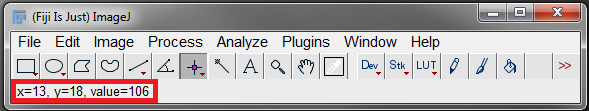
\includegraphics[width=0.7\textwidth]{mod1/figures/pixel-position.png}%
		}
		\medskip
		\captionof{figure}{Pixel position and value.}\label{fig:pixel-position}
		\end{center}
	\end{minipage}
	
	\item While the interpolation helps to visually estimate the 150\% re-sampling in the vertical and diagonal lines, you can see that the original data has been changed.
	\item Try other values for the resizing and observe the results.
\end{enumerate}
\end{taskbox}

As you should have observed, the bilinear interpolation leads to gray values appearing in the previously black-and-white image. Fiji supports the bilinear and the bicubic interpolation. Both interpolation algorithms sample pixel values surrounding each pixel to calculate the pixel value at the given position\footnote{For more information, Wikipedia has entries for bilinear and bicubic interpolations.}. 

Let us go back to our main question of making figures for a manuscript that we want to publish. PNAS recommends a minimum resolution of 300 DPI for color images and further suggests not to use interpolation when changing the size of the image. What should we do with our microscope images? Following guidelines should help you decide what to do:

\begin{itemize}
	\item Best practice: \emph{no image resampling ever} (e.g., see recommendations of the Journal of Cell Biology). Usually, you have enough pixels (>1000 x 1000 pixels), allowing you to choose an image size within your figure that is sufficient. For example, a 1000 x 1000 pixel image at 300 DPI results in about 130 pixels/cm -- you can choose a single column of 89 mm width (Nature requirements again) to display this image. If you then adjust the size of the image in your graphics software, you will only increase/decrease the size of each pixel (like the zoom tool) without resampling.
	\item Never resample more than once during image processing.
	\item Do the resampling at the end, after all other image manipulations and quantifications have been done.	
	\item Report any resampling procedures, including the original image size, pixel dimensions and the interpolation method.
	\item Most journals allow supplementary original data - a good way to present the raw, unfiltered data. Also, there is increasing interest to provide platforms that allow you to publish raw data (e.g. Figshare\footnote{www.figshare.com, an online digital repository - free to upload and free to access; as of 13.10.2014})
	\item Most important if you really have to resample: Convince yourself (and your lab-mates) that the original image and the re-sampled image convey the same information.
\end{itemize}

Fiji also has the option to directly interpolate the image to a given size and DPI (PPI!) using \texttt{[Image > Adjust > Scale To DPI]}. Using this function, you do not have to calculate the values yourself using the \texttt{[Adjust Size]} function (Fig. \ref{fig:scale-to-dpi-dialog}).
\begin{figure}[!h]
	\centering
		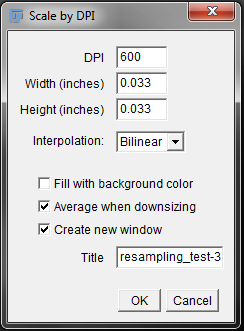
\includegraphics[width=0.3\textwidth]{mod1/figures/scale-to-dpi-dialog.png}
	\caption{Scale to DPI dialog.}
	\label{fig:scale-to-dpi-dialog}
\end{figure}

\newpage
\section{Bit-Depth \& Computer Number Representations}

We already introduced the term bit-depth that describes the range of values that can be represented at each pixel. When we refer to the possible values of each pixel, we use the terms brightness or intensity in the course context. It is very likely that you already encountered the words \emph{bit}, \emph{bits}, (kilo-, mega-, giga-)\emph{bytes} somewhere: 32/64-bit computers, 8/16-bit microscopy images or 50 Mbit/s internet connection speed.

A \emph{bit} is the elementary unit of binary numbers and its possible values are 0 and 1. Electronic devices code and store information with binary numbers because binary states (0 and 1) can easily be implemented in electronics\footnote{While this statement is true, it leaves out any details. However, there are plenty of resources on the web if you are really interested why and how bits are used.}. If you have two bits, you can represent 4 different states (00, 01, 10, 11). In general, if you have \textbf{n} bits, you can represent \textbf{2\textsuperscript{n}} different states. Therefore, 8 bits allow you to represent 256 (2\textsuperscript{8}) different brightness values and 16 bits already 65536 (2\textsuperscript{16}) different values. The higher the bit-depth of our image, the more gray-levels can be represented between black (0) and white (Maximum value). One \emph{byte} consists of 8 bits (historic and convenience reasons). One kilobyte is a multiple of a byte, either 1000 bytes or 1024 bytes; this can be confusing and usually depends on the context. The same is true for further multiples, such as mega-, giga-, tera-, and petabytes.

Similar to choosing an appropriate pixel size (see section \ref{sec:mod1-samplingrate}), we also have to make choices regarding the pixel intensity values during acquisition:
\begin{itemize}
	\item \emph{Bit-depth:} During image acquisition, we round the brightness values found in our samples into a certain number of levels that our chosen bit-depth can represent. For example, if we have 300 distinct brightness levels in our sample and we choose an 8-bit bit-depth, we cannot represent all 300 values (we only have 256 levels!). In this case, the 300 distinct values are rounded to the nearest level that can be represented. Pixels that have different intensities in our sample get rounded to the same values and the differences are lost. In practice, we do not worry about rounding errors during image acquisition -- we usually only have to make the choice between a low bit-depth (8-bit) and a higher bit-depth (12/16-bit). This is discussed in section \ref{sec:bitdepth-choice}. However, rounding errors can present problems during image processing. This is discussed in later chapters.
	\item \emph{Data saturation / clipping: } When you take images on a microscope, you usually set the laser output power, detector gain and detector offset for every image. The reason is that whatever bit-depth we chose, we want the brightest pixels just around the maximum value that can be represented by our bit-depth range and the darkest pixels just around zero. If we use the wrong settings and pixels are saturated/clipped, we loose information about the brightest and darkest parts of our sample. This can prevent further analysis of our data! Clipping can also occur during image processing as you will see in a few minutes.
\end{itemize}

The most common image bit-depths that you can generate with microscopes and that are supported in Fiji are:
\begin{itemize}
	\item 8-bit images that can display 256 gray levels with whole numbers (Integers).
	\item 16-bit images that can display 65536 different gray levels with whole numbers (Integers).
\end{itemize}

In addition, there is a 32-bit image format that allows you to display 2\textsuperscript{32} gray levels with real numbers. However, this format is a little bit more tricky to use as many functions in Fiji do not handle this bit-depth properly.

When you prepare your figures, bit-depth is usually not a big issue. However, you have to be careful when you export/import images using various file formats -- some common file formats only support 8-bit bit-depth and you have to make sure that you convert appropriately.

\newpage
\begin{taskbox}{Bit-Depth Conversion}
\begin{enumerate}
	\item Open the image beads.tif from mod1/data using \texttt{[File > Open]}. Duplicate the image with \texttt{[Image > Duplicate...]}. Choose the line selection tool and draw a line through one of the bright spheres in the image (Fig. \ref{fig:line-roi-example}).	
	
	\begin{minipage}[t]{\linewidth}
		\begin{center}
		\adjustbox{valign=t}{%
			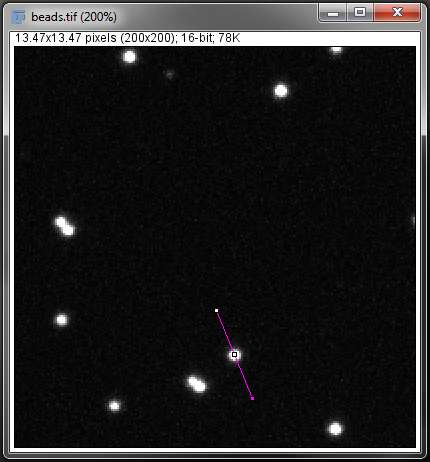
\includegraphics[width=0.5\textwidth]{mod1/figures/line-roi-example.png}%
		}
		\medskip
		\captionof{figure}{A line ROI through one of the beads.}\label{fig:line-roi-example}
		\end{center}
	\end{minipage}
	
	\item In the next step, we will look at the intensity (brightness) distribution along this line. For this, do \texttt{[Analyze > Plot Profile]} (Fig. \ref{fig:plot-profile-example}). You should observe that the gray value (y-axis) ranges from 0 to 65535 and that the curve looks cut at the upper end - this means that we have \emph{saturated} pixels, i.e. we cannot resolve any differences between these saturated pixels although the shape of the curve would suggest intensity changes. The [Plot Profile] function allows you to list (show), save and copy the values. If you click on \texttt{[Live]}, you can change the line ROI and the plotted profile will update. Try the update by drawing a line somewhere on the background and then again through a bead. Turn the live mode off again by another click on the button. 

\begin{minipage}[t]{\linewidth}
		\begin{center}
		\adjustbox{valign=t}{%
			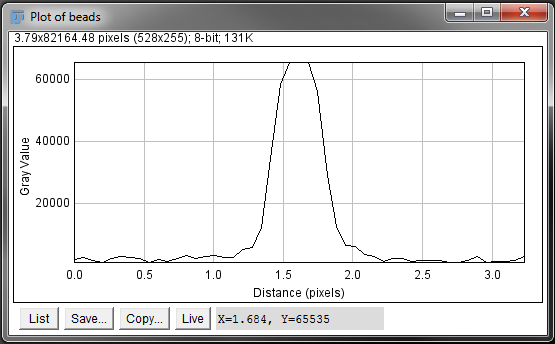
\includegraphics[width=0.5\textwidth]{mod1/figures/plot-profile-example.png}%
		}
		\medskip
		\captionof{figure}{Intensity profile of the line.}\label{fig:plot-profile-example}
		\end{center}
	\end{minipage}

\item Now, we convert the 16bit image to 8bit. First, we make sure that we scale during conversion by \texttt{[Edit > Option > Conversion]}. Then, we use \texttt{[Image > Type > 8-bit]} to convert the image. Make sure that the line ROI is still there and perform the plot profile function again. A second window pops up. Compare the plot profiles of the 8-bit and the 16-bit images. The conversion modified the brightness value (y-value). While the profiles are similar, the scaling is different. The image is scaled according to following equation:
	\[I_{8bit}=\frac{I_{16bit}(x,y)-min(I_{16bit}(x,y))}{max(I_{16bit}(x,y))-min(I_{16bit}(x,y))}*2^8
	\]
with:\\
I\textsubscript{16bit}(x,y): 16bit image\\
I\textsubscript{8bit}(x,y): 8bit image\\
max(I\textsubscript{16bit}(x,y)): maximum value of 16bit image\\
min(I\textsubscript{16bit}(x,y)): minimum value of 16bit image\\
\item Convert the image back to 16-bit and check the intensity values again. In this case, the intensity values are not increased. 
\item The conversion actually looks at the data as it is displayed. Adjust the brightness and contrast to an extreme value using \texttt{[Image > Adjust > Brightness/Contrast...]} (contrast slider to the right edge). Convert the image to 8-bit again. Look at the profile of a bead. You should see that the image only consists of 2 intensities: 0 and 255. As you saw, it is important to reset the brightness and contrast display before converting the image.
\end{enumerate}

\end{taskbox}

\subsection{Choice of Bitdepth}
\label{sec:bitdepth-choice}

The choice whether to use a low or high bit-depth depends on the application. Of course you could always use the maximum bit-depth available (to be on the safe side). However, this increases the amount of data you acquire. For example, going from 8-bit to 16-bit doubles the required harddisk space. In addition, image processing might be much slower as well! A typical application where a lower bit-depth is sufficient is where you have a very bright signal (signal-noise ration very good) and you just want to identify cells (vesicle, nuclei, ...) for counting or shape analysis. On the other hand, if you want to analyze bright regions as well as darker regions, or need precise intensity comparisons (e.g. for protein density measurements), a higher bit-depth is recommended.

\section{Image Dimensions}

Up to now, we just looked at 2-dimensional images, where each pixel \emph{p} can be identified by its spatial coordinates, its position along both axes \emph{p(x,y)}. In microscopy, we often deal with more dimensions, common scenarios are:

\begin{itemize}
	\item \textbf{3D z-stacks:} A single acquisition of a 3D volume. The additional dimension is the depth of the section. Each pixel \emph{p} can be identified by \emph{p(x,y,z)}.
	\item \textbf{3D time-series:} A sequence of 2D image acquisitions. The additional dimension is the time of the acquisition. Each pixel \emph{p} is identified by \emph{p(x,y,t)}. 
	\item \textbf{3D multi-channel images:} A 2D image is acquired with >1 color channel (multiple fluorophores). The additional dimension is the color. Each pixel is identified by \emph{p(x,y,c)}.
	\item \textbf{4D images:} a combination of 4 already discussed dimensions: z-stacks with multiple color channels, sequence of z-stacks over time or 2D multicolor image over time.
	\item \textbf{5D images:} a combination of all discussed dimensions: sequence of z-stacks with multiple color channels over time. Each pixel \emph{p} is identified by \emph{p(x,y,c,z,t)}.
\end{itemize}

Fiji allows you to work with all these image types and we will discuss those methods and possible ways to visualize these data in publications in the following sections.

\subsection{3D stacks}

For historical reasons, Fiji (ImageJ) has two different structures to handle 3D data. At first, ImageJ used \emph{stacks} to support 0-3 dimensions. This was done to z-slices or time points. To be more flexible, \emph{hyperstacks} were introduced to support 0-5 dimensions. For compatibility reasons, both structures co-exist at the moment, but the distinction is disappearing with the hyperstack becoming the standard structure to represent multi-dimensional data. As you will see, hyperstacks are used when importing microscopy file formats. If a pixel \emph{p} defined by three spatial dimensions \emph{p(x,y,z)}, we call the pixel \emph{voxel} (volume element).

\begin{taskbox}{Viewing a 3D Stack}

\begin{enumerate}
	\item Open the file flybrain-template.tif in /mod1/data. This is an 8-bit gray-scale z-stack, showing a standard template of a fly brain. You should see that there is a slider below the image to go through individual z-sections of the stack. 
	\item If the image looks too bright or dark, adjust the brightness (\texttt{[Image > Adjust > Brightness/Contrast...]}).
	\item Click on the start animation button left to the slider to start an automatic stepping through the sections (Fig. \ref{fig:stack_animation_button} similar to a video). Clicking on the button again, pauses the animation (button icon changes accordingly).
	
	\begin{minipage}[t]{\linewidth}
		\begin{center}
		\adjustbox{valign=t}{%
			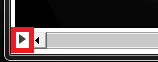
\includegraphics[width=0.3\textwidth]{mod1/figures/stack-animation-button.png}%
		}
		\medskip
		\captionof{figure}{Start stack animation.}\label{fig:stack-animation-button}
		\end{center}
	\end{minipage}
	
	\item Using the stack toolbar (Fig. \ref{fig:stack-toolbar}), you can \texttt{[Start Animation]} and \texttt{[Stop Animation]} as well.
	
	\begin{minipage}[t]{\linewidth}
		\begin{center}
		\adjustbox{valign=t}{%
			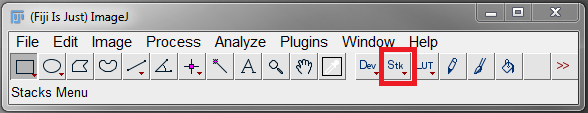
\includegraphics[width=0.7\textwidth]{mod1/figures/stack-toolbar.png}%
		}
		\medskip
		\captionof{figure}{Stacks toolbar.}\label{fig:stack-toolbar}
		\end{center}
	\end{minipage}
	
	\item Use the \texttt{[Animation Options]} from the stack toolbar to increase the animation speed to 20 fps (frames-per-second) and loop back and forth. The animation should look much smoother now (Fig. \ref{fig:animation-options-dialog}).
	
	\begin{minipage}[t]{\linewidth}
		\begin{center}
		\adjustbox{valign=t}{%
			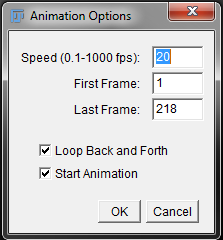
\includegraphics[width=0.4\textwidth]{mod1/figures/animation-options-dialog.png}%
		}
		\medskip
		\captionof{figure}{Stacks toolbar.}\label{fig:animation-options-dialog}
		\end{center}
	\end{minipage}
	
	\item When you want to use an animation of the stack in a presentation, you can save the stack as an avi using \texttt{[File > Save As > AVI...]}.
	
\end{enumerate}

\end{taskbox}

It is possible that the image data you import has the dimensions mixed up. If the data is a stack, you can use \texttt{[Image > Properties]} to reorder channels, slices and frames. However, it is more flexible to convert the stack to a hyperstack and perform re-ordering on the hyperstack.

\begin{taskbox}{Order of Dimensions}

\begin{enumerate}
	\item Open the file flybrain-template.tif in /mod1/data if it is not still open.
	\item Use \texttt{[Image > Hyperstacks > Stack to Hyperstack...]} to convert the stack to a hyperstack. In our test image, the order, channels, slices and frames should be detected correctly. 
	\item Now, you can easily re-order the dimensions of the hyperstack using \texttt{[Image > Hyperstacks > Re-order Hyperstacks...]}. Although this does not make any sense, change the z-dimension to a time dimension. As you can see, from the user perspective, this does not change anything at the moment.
\end{enumerate}

\end{taskbox}

Fiji offers many ways to manipulate (hyper)stacks. You can concatenate, combine, interleave, insert or split stacks; convert images to stacks and back, remove and add slices, make substacks, create a montage or generate a stack from a montage. These functions can be found under \texttt{[Image > Stacks]} and especially \texttt{[Image > Stacks > Tools]}. 

\begin{taskbox}{Manipulating Stacks -- Creating a Montage}
A common way 3-dimensional data is presented (typically along time or z-axis) is the montage view.

\begin{enumerate}
	\item Open the file flybrain-template.tif in /mod1/data if it is not still open.
	\item Use \texttt{[Image > Stacks > Make Montage...]}. In the dialog, set \texttt{[Columns]} and \texttt{[Rows]} to 5, \texttt{[First Slice]} to 100, \texttt{[Last Slice]} to 124, change the \texttt{[Border Width]} to 1 pixel and tick \texttt{[Label Slices]} (Fig. \ref{fig:make-montage-dialog}).
	
	\begin{minipage}[t]{\linewidth}
		\begin{center}
		\adjustbox{valign=t}{%
			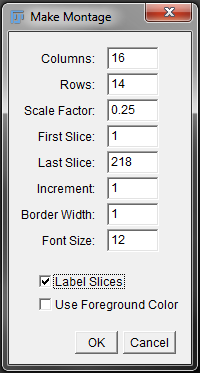
\includegraphics[width=0.4\textwidth]{mod1/figures/make-montage-dialog.png}%
		}
		\medskip
		\captionof{figure}{Make Montage Dialog.}\label{fig:make-montage-dialog}
		\end{center}
	\end{minipage}
	
	\item You can see how easy it is to create a custom montage view, play with the different options, e.g. \texttt{[Increment]}.
\end{enumerate}

\end{taskbox}

\begin{taskbox}{Manipulating Stacks -- Creating an Insert}
We now want to do something more complicated: let's say we want to show a detail of the flybrain, e.g. the central complex or the optic lobes. To help viewers, we want to put a little version of the complete brain in the corner of our 3D image as an overview. How would you proceed?

\begin{enumerate}
	\item Open the file flybrain-template.tif in /mod1/data if it is not still open.
	\item Use the rectangle tool to select an interesting part of the brain that you want to highlight. Duplicate the complete stack using \texttt{[Image > Duplicate]}, this will only duplicate the part you selected. 
	\item Use \texttt{[Image > Adjust > Size...]} to create an image with 1024 pixel width and no interpolation.
	\item Go back to our original image of the fly brain and use \texttt{[Image > Scale...]} to reduce the image size to 20\% (x, y) with bilinear interpolation.
	\item The insert is created with \texttt{[Image > Stacks > Tools > Insert...]}. Make sure you use the detailed view of brain as \texttt{[Destination]} and the overview as \texttt{[Source]}. \texttt{[X-Location]} and \texttt{[Y-Location]} can remain 0 (Fig. \ref{fig:stack-inserter-dialog}).
	
	\begin{minipage}[t]{\linewidth}
		\begin{center}
		\adjustbox{valign=t}{%
			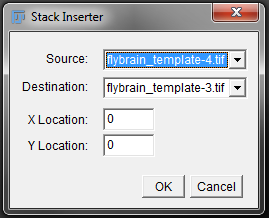
\includegraphics[width=0.4\textwidth]{mod1/figures/stack-inserter-dialog.png}%
		}
		\medskip
		\captionof{figure}{Stack Inserter Dialog.}\label{fig:stack-inserter-dialog}
		\end{center}
	\end{minipage}
	
	\item Again, a very easy procedure -- explore further stack operations on your own.
\end{enumerate}

\end{taskbox}

\subsection{Color images}

So far, we only analyzed images with one color channel (grayscale), i.e. at each spatial position, we only had one pixel with one value. In microscopy, we often encounter multi-channel images where each channel corresponds to one modality. One channel for each fluorophore intensity, a channel for a DIC image or even a channel that does not represent brightness but for example fluorophore lifetime. Outside microscopy, we also usually encounter color images, these are often RGB images that consist of red, green and blue 8-bit channels. Again, publisher demands on the color usage varies, sometimes they demand that the RGB color space you usually work with on your computer is converted to the CMYK color space that is typically used in print. Luckily, as the primary source for distributing and viewing a publication are various digital devices, conversion demands become less common. 

\minisec{Color models}
Outside microscopy, two colorspaces are very common:
\begin{enumerate}
	\item RGB (Red Green Blue)\\A single RGB image has three, fixed color channels: red, green and blue. Each of those have a fixed bit-depth of 8-bit, resulting in a single RGB image with 24-bit. These colors have been chosen as computer screens generate colors by mixing red, green and blue light and therefore, RGB images directly determine how much of each color to use but are device dependent (actually, RGB is based on human color perception).
	\item CMYK (Cyan Magenta Yellow Key)\\A single CMYK image is based on four colors: cyan, magenta, yellow and black. The color model is primarily used in printing, but is device-dependent as well. When you want to publish a manuscript, it is very likely that you will be asked to convert your figures to the CMYK color space. This can be done with Fiji using existing Plugins, but it might be better to perform the conversion for the total final figure when all other editing has been finished. As the online versions of publications have become much more important than the actual prints, efforts to produce color-true conversions for printing become much less important.
\end{enumerate}

\newpage
\begin{taskbox}{RGB Images}

\begin{enumerate}
	\item Open the file muscle-cell.tif in /mod1/data\. This image was taken from a publication in Nature Cell Biology 5, 598(2003); Cell of the Month: The vascular smooth muscle cell cytoskeleton; Mario Gimona; DOI:10.1038.ncb0703-598. This RGB image shows mouse smooth muscle cell with fluorescent labels of the cytoskeleton. Use \texttt{[Image > Show Info...]} for details about this image.
	\item Use \texttt{[Image > Adjust > Brightness/Contrast]} and change the slider values. Observe that this operation affects all colors simultaneously. Reset the changes.
	\item We now split the red, green and blue channels of the RGB image with \texttt{[Image > Color > Split Channels]}. Three windows appear, each showing the respective color content. 
	\item Let's combine these channels again with \texttt{[Image > Color > Merge Channels]}. The merge-function gives us many options to create a merged image (Fig. \ref{fig:merge_channels_dialog}). Do not set any options and use the same color channels.
	
	\begin{minipage}[t]{\linewidth}
		\begin{center}
		\adjustbox{valign=t}{%
			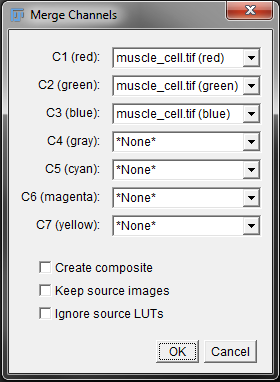
\includegraphics[width=0.4\textwidth]{mod1/figures/merge-channels-dialog.png}%
		}
		\medskip
		\captionof{figure}{Merge Channels Dialog.}\label{fig:merge-channels-dialog}
		\end{center}
	\end{minipage}
	
	\item Now split again and merge back, but with option \texttt{[Create composite]} ticked. This creates a slider below the image, indicating that we created a three-layered stack, one layer for each color.  
	\item The composite image allows us to work on each channel separately. Perform \texttt{[Image > Color > Channels Tool...]}. In this dialog, you can select individual channels in composite mode or view individual channels in Color/Grayscale mode (Fig. \ref{fig:channels-tool-dialog}). Try out the different settings.
	
		\begin{minipage}[t]{\linewidth}
		\begin{center}
		\adjustbox{valign=t}{%
			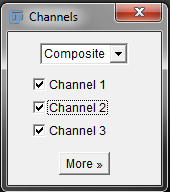
\includegraphics[width=0.4\textwidth]{mod1/figures/channels-tool-dialog.png}%
		}
		\medskip
		\captionof{figure}{Channels Tool Dialog.}\label{fig:channels-tool-dialog}
		\end{center}
	\end{minipage}
	
	\item Try to perform already know operations on just one color channel, e.g. Adjust the brightness (you can see that the little histogram changes color when you change the channel!).
\end{enumerate}

\end{taskbox}

\begin{taskbox}{Convert RGB to CMYK -- Extending Fiji with Plugins}
Although Fiji has a great core functionality included, the power of this tool can only be appreciated with the many existing macros and plugins. While some plugins are already included in the Fiji distribution, you most likely will encounter some function you need that is not included -- and if this is a common task it is very likely that someone already solved this problem. 

\begin{enumerate}
	\item Convert the composite image back to a RGB image with \texttt{[Image > Color > Stack to RGB]}.
	\item We now want to convert the RGB image into a CMYK image for publication. However, Fiji is not able to do so and we have to extend the functionality. A quick search ('imagej convert to cmyk') shows that, fortunately, Stephan Saalfeld and Wayne Rasband wrote a plugin for this (two names you might encounter more often).
	\item You can find the file RGB\_to\_CMYK.class in the folder mod1/data/. Installing this plugin is very easy, just drag and drop the file onto the main Fiji window. You are asked to save the file in the plugins directory of Fiji. 
	\item Convert the image to CMYK with \texttt{[Plugins > RGB to CMYK]}.
\end{enumerate}

\end{taskbox}

\minisec{Lookup Tables}
For a computer, an image is a matrix with the same dimensions as the image and the range of possible values at each matrix position are determined by the bit-depth. A \emph{lookup table (LUT)} maps these values to a color/brightness that is displayed on the screen. Often, the LUT is simply called \emph{colormap}. The default LUT is gray-scale that, in an 8-bit image, assigns black to zero and white to 255. Intermediate values are represented as gray-levels and the same idea applies to any bit-depth.
The advantage using a LUT is obvious; we can create arbitrary LUTs with any coloring we want. These colored LUTs are called 'pseudo-color'. These LUTs are typically used to indicate fluorophore emission wavelengths but are sometimes changed to emphasize certain aspects of the data.

Figure \ref{fig:lookup-tables} shows the LUTs available in Fiji, the figure was created by the command \texttt{[Image > Color > Display LUTs]}. Very common LUTs are \emph{grayscale}, \emph{spectrum}, \emph{fire} and \emph{physics}.

\begin{taskbox}{Exploring Lookup Tables}

\begin{enumerate}
	\item Open the image beads.tif in /mod1/data. You can look at the LUT of the current image with \texttt{[Image > Color > Show LUT]} which is the standard linear grayscale LUT you have already seen.
	\item Change the LUT using \texttt{[Image > Color > Edit LUT...]}. Click on the top-left dark value and change the color from black to blue,  select the white entry from the bottom right and change the color to red (Fig. \ref{fig:lut-editor}).
	
	\begin{minipage}[t]{\linewidth}
		\begin{center}
		\adjustbox{valign=t}{%
			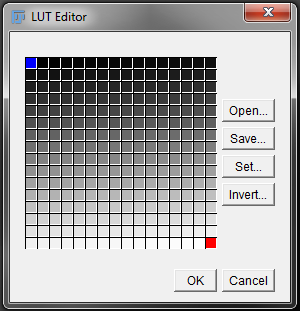
\includegraphics[width=0.4\textwidth]{mod1/figures/lut-editor.png}%
		}
		\medskip
		\captionof{figure}{LUT Editor.}\label{fig:lut-editor}
		\end{center}
	\end{minipage}
	
	\item Look at the image. Does it look familiar? This is the HiLo LUT that is often used in microscopy to optimize parameters for acquisition (emitted light, gain, offset). You can obtain the same image by selecting the HiLo LUT in Fiji (Fig. \ref{fig:lut-tool}).
	
	\begin{minipage}[t]{\linewidth}
		\begin{center}
		\adjustbox{valign=t}{%
			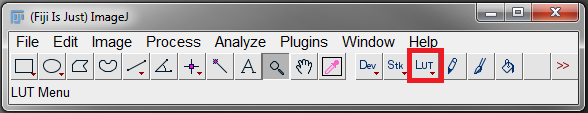
\includegraphics[width=0.4\textwidth]{mod1/figures/lut-tool.png}%
		}
		\medskip
		\captionof{figure}{LUT Tool.}\label{fig:lut-tool}
		\end{center}
	\end{minipage}
	
	\item Close the image and open the file cell-colony.tif in /mod1/data. Change the LUT to Spectrum using \texttt{[Image > Lookup Tables > Spectrum]}.
	\item Display the current LUT of the image. Try out different available LUTs and display their profile.
\end{enumerate}

\end{taskbox}

\begin{figure}[!ht]
	\centering
		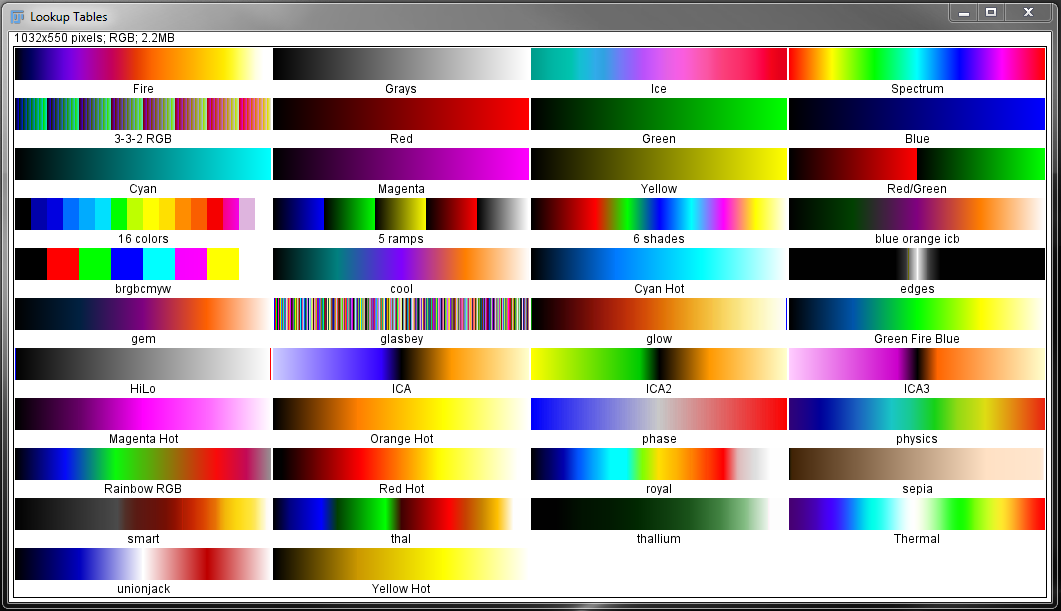
\includegraphics[width=0.80\textwidth]{mod1/figures/lookup-tables.png}
	\caption{Lookup Tables in Fiji}
	\label{fig:lookup-tables}
\end{figure}

\minisec{A short note about colors in publications}
There is plenty of literature around discussing the best colormaps and general rules one should apply when using colors in scientific publications. We do not want to enter this, sometimes heated, debate, as color choice in microscopy usually comes naturally based on the wavelengths. Nevertheless, we want you to get a feeling why this debate is going on and provide two examples: \emph{Color Bias} and \emph{Color Blindness}. Color bias refers to the problem that poor color choices can introduce a biased view of our data. For example, when we change the grayscale LUT to a spectrum LUT, relative changes of intensity can be obscured. Color blindness addresses the issue that microscopy images, especially illustrating colocalization, are often presented with red and green (all following information on color blindness is taken from \cite{wong2011}). However, a substantial number of people are affected by various forms of color blindness (about 8\% of male Europeans). Therefore, it is very likely that you will have reviewers for your manuscripts or audience in your talk that are color blind. One option to adjust your images is simply to replace the red with magenta.

\begin{taskbox}{Effects of LUT Changes}

\begin{enumerate}
	\item Open the image muscle-cell.tif in /mod1/data. 
	\item Simulate color-blindness with \texttt{[Image > Color > Simulate Color Blindness]}. This function only works on an RGB image. 
	\item Use \texttt{[Image > Color > Replace Red with Magenta]} to exchange colors and then simulate color-blindness again. Color differences are much more obvious in the second image.
	\item go back to the original image of the muscle and split the channels.
	\item Duplicate the window containing the blue channel information.
	\item Change the LUT to spectrum and discuss the differences between the gray and spectrum LUTs.
\end{enumerate}

\end{taskbox}

\begin{taskbox}{Calibration Bars}
A calibration bar is typically added to a figure when intensity comparisons are made. A calibration bar indicates which color corresponds to which brightness. This is especially important when you use LUTs with more than one color or when you use a single color LUT where the change in intensity is not linear ('gamma').

\begin{enumerate}
	\item Open the image fibroblast-sim.tif in /mod1/data. 
	\item Adjust Brightness/Contrast and select a LUT you like.
	\item Add a calibration bar with [Analyze > Tools > Calibration Bar...]. In the dialog, choose a location, fill color, label color, number of labels, asf. (Fig. \ref{fig:calibration-bar-dialog}). Note that this calibration bar shows the brightness settings you just applied and that you cannot change those now.	
	
	\begin{minipage}[t]{\linewidth}
		\begin{center}
		\adjustbox{valign=t}{%
			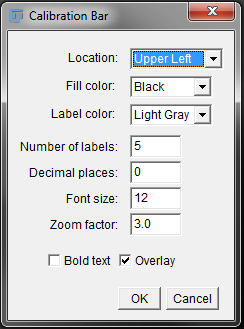
\includegraphics[width=0.4\textwidth]{mod1/figures/calibration-bar-dialog.png}%
		}
		\medskip
		\captionof{figure}{Calibration Bar Dialog.}\label{fig:calibration-bar-dialog}
		\end{center}
	\end{minipage}
	
\end{enumerate}

\end{taskbox}

\newpage
\subsection{4D/5D stacks}
It is common that the data you acquire on microscopes has more than 3 dimensions. In this section, we will first discuss how you work with these data before we will discuss the problem of presenting this data in a figure.

With the hyperstack data format, representation of 4D and 5D data is very similar. Basically, sliders are added to the image window. However, you have to keep the order of dimensions in mind. Common dimension order is XYCZT, however this order might be different when you import data -- doublecheck when importing!

\begin{taskbox}{Working with 5D Data}
To illustrate working with 5D data, we will import a sequence of files that are labeled with \_t000\_z000\_c000 and increasing numbering. The sequence of files has been generated from the standard Fiji sample Mitosis \texttt{[File > Open Samples > Mitosis (26 MB, 5D stack)]}. This data shows Drosophila S2 cell expressing GFP-Aurora B and mCherry-tubulin fusion protein undergoing mitosis (Courtesy of Eric Griffis).

\begin{enumerate}
	\item Go to \texttt{[Plugins > Bio-Formats > Bio-Formats Importer]} and select the first image in the folder /mod1/data/mitosis.
	\item The Bio-Formats import options dialog shows up, make sure to select [Group files with similar names].
	\item In the dialog, you can choose how to stitch the files (Fig. \ref{fig:bioformats-file-stitching}). We select Pattern. This parses the file based on: mitosis\_t0<01-51>\_z00<1-5>\_c00<1-2>.tif. <> denote the range of the import, e.g. we could only select one channel, or any other substack.
	
	\begin{minipage}[t]{\linewidth}
		\begin{center}
		\adjustbox{valign=t}{%
			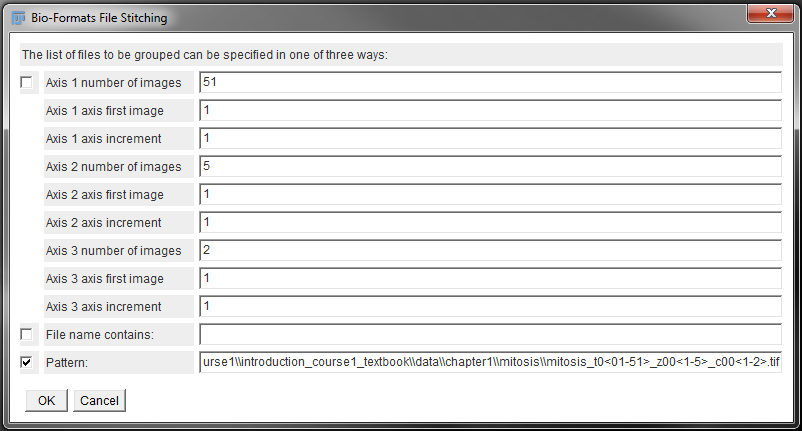
\includegraphics[width=0.8\textwidth]{mod1/figures/bioformats-file-stitching.png}%
		}
		\medskip
		\captionof{figure}{Bio-Formats File Stitching Dialog.}\label{fig:bioformats-file-stitching}
		\end{center}
	\end{minipage}
	
	\item The imported image shows three sliders: channel (2), z-position(5), time-stamps(51). Browse through the image, adjust Brightness if necessary. On thing to notice is that we lost information about the z-spacing, distance between time-stamps or channel colors.
\end{enumerate}

\end{taskbox}

\subsection{Visualizing Multidimensional Data}
You already worked with the most basic visualization of multidimensional data that only displays two dimensions at a time. In this view, you can browse through the dimensions by adjusting the sliders. Another view we already discussed is the image montage. Both of these visualizations are also valid options to present the data in a figure. In general, visualizing multi-dimensional data is non-trivial, as we are constrained by the physical limitations of our visual sense. In this section, we will look at some common visualization techniques for multi-dimensional microscopy data that are useful to highlight certain aspects of your data in a figure.

\begin{taskbox}{Projection (Dimensionality reduction)}
The first visualization we will explore is the projection. In a projection, data is summarized along one axis (dimension). A typical case is the maximum intensity projection of the z-axis of a 3D stack, resulting in a 2D image where each pixel represents the maximum value that was found in this \emph{(x,y)} position along \emph{z} - which is then used for the manuscript. In Fiji, you can choose between the minimum, average or maximum intensity projection and the sum, standard deviation or median of each pixel along \emph{z}. Remember that you can swap dimensions with \texttt{[Image > Hyperstack > Re-order Hyperstack]}.

\begin{enumerate}
	\item Open the image GMR-10A12-AE-01.tif from /mod1/data. This image shows the expression patterns of a GAL4 line, displayed on a standardized fly brain template (credits belong to the Rubin-lab, JFRC (Arnim Jennet) and The Virtual Fly Brain). Try to estimate the expression pattern (green) by going through \emph{z} using the slider. 
	\item In this case, we might decide a z-projection is helpful to quickly determine whether the expression pattern is of interest. We can perform the projection with \texttt{[Image > Stacks > Z Project...]}, choosing Max Intensity (Fig. \ref{fig:z-projection-dialog}).
	
	\begin{minipage}[t]{\linewidth}
		\begin{center}
		\adjustbox{valign=t}{%
			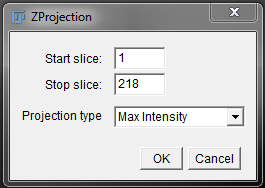
\includegraphics[width=0.4\textwidth]{mod1/figures/z-projection-dialog.png}%
		}
		\medskip
		\captionof{figure}{Z Projection Dialog.}\label{fig:z-projection-dialog}
		\end{center}
	\end{minipage}
	
	\item Explore various projections on the stack created from the file sequence in mod1/data/mitosis/.
\end{enumerate}

\end{taskbox}

\begin{taskbox}{Orthogonal View}
Another very common visualization is the orthogonal view. In this view, two additional windows are created that are linked to the current slider position of the 2D view. These windows show the XZ and YZ position. This visualization can be useful if you want to present the intensity profiles in 3D data while presenting overview images for the orientation of the reader at the same time.

\begin{enumerate}
	\item Open the stack GMR-10A12-AE-01.tif from mod1/data/ if it is not already open. Show the orthogonal view with \texttt{[Image > Stacks > Orthogonal Views]}. Try scrolling through the axes to get a feeling for this view.
\end{enumerate}

\end{taskbox}

\newpage
\begin{taskbox}{Color Coding}
One option to add a third dimension on a 2-dimensional plot is to somehow code the information; e.g. using different colors for z-depth or time. This can be useful when the data is structured along on axis, e.g. different layers of cells within a tissue, axons growing into other tissue parts or vesicles moving around over time.

\begin{enumerate}
	\item Open the image fake-tracks.tif from /mod1/data (another Fiji sample image). We use a fake file to better illustrate how the color coding works, but you can apply it to any 3D data for further testing. Perform [Image > Hyperstacks > Temporal-Color Code] and select a LUT of your choice (Fig. \ref{fig:color-code-dialog}).
	
	\begin{minipage}[t]{\linewidth}
		\begin{center}
		\adjustbox{valign=t}{%
			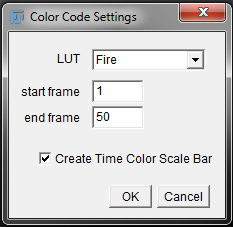
\includegraphics[width=0.4\textwidth]{mod1/figures/color-code-dialog.png}%
		}
		\medskip
		\captionof{figure}{Temporal Color Code Dialog.}\label{fig:color-code-dialog}
		\end{center}
	\end{minipage}
	
	\item Compare the color-coded image with the original time-series.
\end{enumerate}

\end{taskbox}

\begin{taskbox}{Generating a Kymograph Plot}
A Kymograph is an visualization to present a dynamic process in a single image where movements along a line are plotted for all time-frames in a stack (\emph{x-t} plot). Therefore, it is also a way to deruce dimensionality. They are common to show cellular components moving along a some path (e.g. mitochondria moving along an axon or cells migrating in reference to a body axis during development).

\begin{enumerate}
	\item Open the stack axon-mitos.tif from /mod1/data (Image by Arun Akondadi, Rugarli Lab, University of Cologne). Adjust Brightness. This image shows mitochondria moving along an axon.
	\item This image has a problem: the axon was not stained itself, but we can hopefully reconstruct the axon path by the positions of the moving mitochondria. For this, perform a maximum projection over time.
	\item The maximum-intensity image helps a lot to estimate the axon position in the image. Right-click on the [Line-Tool] to change the Straight Line to a Segmented Line (Fig. \ref{fig:segmented-line-selection}). Use the segmented line to trace the axon path. A double-click ends the line.	
	
	\begin{minipage}[t]{\linewidth}
		\begin{center}
		\adjustbox{valign=t}{%
			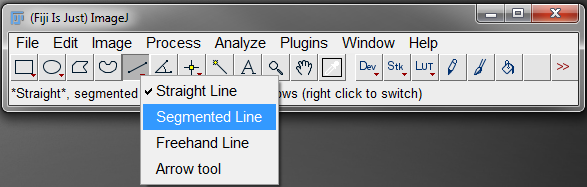
\includegraphics[width=0.6\textwidth]{mod1/figures/segmented-line-selection.png}%
		}
		\medskip
		\captionof{figure}{Segmented Line Tool.}\label{fig:segmented-line-selection}
		\end{center}
	\end{minipage}
	
	\item Go to the original stack and do \texttt{[Edit > Selection > Restore Selection]}. This restores the line we just selected on the maximum projection on the stack.
	\item Use \texttt{[Image > Stack > Reslice]} to generate the Kymograph. For display reasons, you can also invert the image with \texttt{[Edit > Invert]} and Adjust the Brightness.
	\item If the line was placed correctly, you should see something similar to Fig. \ref{fig:kymograph}. The kymograph helps to distinguish stationary mitochondria and we can sometimes even distinguish anterograde from retrograde movement (in reference to soma).	
	
	\begin{minipage}[t]{\linewidth}
		\begin{center}
		\adjustbox{valign=t}{%
			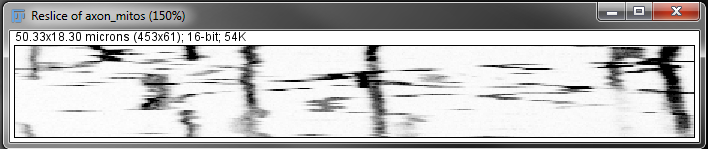
\includegraphics[width=0.6\textwidth]{mod1/figures/kymograph.png}%
		}
		\medskip
		\captionof{figure}{Example Kymograph.}\label{fig:kymograph}
		\end{center}
	\end{minipage}
	
\end{enumerate}

\end{taskbox}

\newpage
\begin{taskbox}{3D View}
Instead of trying to visualize our data in 2 dimensions, we can also visualize in 3D using the 3D viewer in Fiji. For visualizations in 3D, several display options are common: Volume, Orthoslice, and Surface. While this choice is obviously not available for printed figures, online publishing of supplementary videos can be a good option to present your data.

\begin{enumerate}
	\item Open the stack GMR-10A12-AE-01.tif from /mod1/data if it is not already open. Select the 3D viewer with [Plugins > 3D Viewer]. In the options dialog (Fig. \ref{fig:3D-viewer-dialog}), select the image and display as a volume.	
	
	\begin{minipage}[t]{\linewidth}
		\begin{center}
		\adjustbox{valign=t}{%
			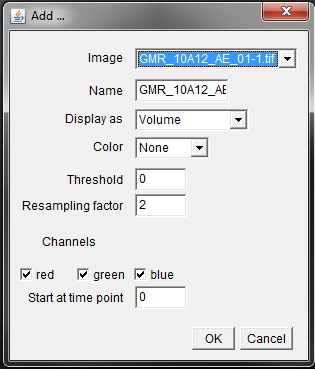
\includegraphics[width=0.3\textwidth]{mod1/figures/3D-viewer-dialog.png}%
		}
		\medskip
		\captionof{figure}{3D Viewer Dialog.}\label{fig:3D-viewer-dialog}
		\end{center}
	\end{minipage}
	
	\item Depending on your hardware, this might take a while to display. Try to navigate the 3D view with your mouse. 
	\item Let us try to generate a movie that you can save as an avi file. Use the 3D viewer menu to create a simple 360 degree rotation with \texttt{[View > Record 360 degree rotation]}. This generate a stack that you can now save as a movie using \texttt{[File > Save As > AVI]}. In this dialog, you can set the compression as well as the frame rate (how fast the movie is displayed). For our purposes, we set the compression to uncompressed and the Frame Rate to 15 fps (frames-per-second). Movie generation for journals can also be a tricky thing as they often impose strict size limits and requires specific formats. You often need to adjust the movie size as well as the compression algorithm to adhere to these requirements and the choice of both can be complicated. However, you can usually accept some compression artefacts as movies are often not considered raw data but more of a nice additional visualization. Still, make sure that you adhere to scientific principles and tell specifically how you treated your data to generate the movie.
	\item Further instructions on the 3D viewer can be found at: http://3dviewer.neurofly.de/; the website of the developers (as of 28.10.2014).
\end{enumerate}

\end{taskbox}

\section{File Formats}
File formats are an important, but dry topic. Every time you share data with colleagues or during the manuscript submission process, you have to work with various formats. This section discusses some basics of formats, focusing on formats suitable for microscopy data (and more general image file formats).

An image file consists of two main parts:
\begin{enumerate}
	\item \emph{Header} -- The header contains additional information about your image, such as image type, dimensions, bit-depth, pixel size, microscope settings and general file information. The data in the header is often called \emph{metadata}. Parts of the metadata are as important as the pixel data as they are necessary to interpret the image data (e.g. pixel size, bit-depth). 
	\item \emph{Content} -- The content of an image file consists of the actual pixel data, the matrix with numerical values. 
\end{enumerate}

The way the header and the pixel data are organized is determined by the file format. Many general image file formats exists, common are JPEG, PNG, TIFF or GIF. These formats are read by many different software tools across platforms and allow quick previews in all major operating systems. They are therefore very suitable to view and share image data. However, there are some problems with these file formats when we want to use them to store our scientific image data:
\begin{itemize}
	\item The format \emph{metadata} might not include essential information about our microscopy data (e.g. pixel size).
	\item \emph{Bit-depth} choice can be limited (e.g. GIF only allows 8-bit).
	\item \emph{Multi-dimensional information} might not be supported and extra-dimensions lost when converted (limits apply to all standard formats).
	\item The format uses \emph{lossy compression} to shrink file size (e.g. JPEG).
	\item Sometimes, limits on the \emph{maximum number of pixels} in a plane can prevent use for microscopy data.
\end{itemize}

\minisec{Compression}
Compression is used to reduce image file sizes. In general, compression methods can be divided into two types: \emph{loss-less} and \emph{lossy} compression. As the names indicate, the original pixel data cannot be reconstructed if lossy compression is employed (information is lost) and the original data can be reconstructed in lossless compression. A typical example of lossless compression is used in PNG. In this format, compression is achieved by shrinking redundant parts. JPEG and GIF are usually lossy formats. In addition to shrinking redundant parts, these formats also interpolate parts of the image to decrease file size even more.  

\begin{quotation}
	Lossy compression should be avoided to maintain scientific integrity!\\(Unless you know exactly what you are doing)
\end{quotation}

Limitations of general image file formats led many microscope and image processing software manufacturers to develop their own image file formats (LIF, SCN -- Leica, LSM, ZVI -- Zeiss, ND2 -- Nikon, ...). These formats store all important metadata information and the original pixel data (only loss-less compression used). However, the drawback is that you typically need proprietary software to view these files and access all metadata and that another software you want to use for analysis or display might not be able to read the original data file.

\begin{quotation}
	The originally acquired files are the most trustworthy -- this is your original, raw data\\You should always keep these files with appropriate backup solutions\footnote{It is also very likely that the funding agency supporting your research has rules how you treat your original data!}.
\end{quotation}

As you can see, this is a mess for researchers. On the one hand, you want to maintain scientific integrity and adhere to standards concerning your data, but on the other hand, you want to share your data and have easy access for further processing.

Fortunately, the LOCI Bioformats plugin\footnote{http://www.openmicroscopy.org/site/support/bio-formats5/ (as of 24/10/2014)} can import most proprietary file formats and extract most of their metadata in Fiji. There is also significant effort by the Open Microscopy Environment (OME) to provide a standardized file format OME-TIFF that includes rich metadata descriptions suitable for microscopy. This is an ongoing process and if you use this format to store and share data, you have to make sure that all important metadata is actually included.

Journals usually accept common image file formats (if compressed with loss-less compression). I would recommend using a vector graphics program for final figure preparation (think about text/line art) with microscopy images embedded (that have been prepared by e.g. Fiji).

\begin{taskbox}{Using Bioformats}
Let's import a microscope specific file format into Fiji.

\begin{enumerate}
	\item Open the image sted-confocal.lif in /mod1/data by drag/drop or with \texttt{[Plugins > Bio-Formats > Bio-Formats Importer]}.  
	\item In the next dialog, you can select various import options (Fig. \ref{fig:bioformats-import-dialog}). Make sure that you load the data into a Hyperstack and tick the Display metadata option.
	
	\begin{minipage}[t]{\linewidth}
		\begin{center}
		\adjustbox{valign=t}{%
			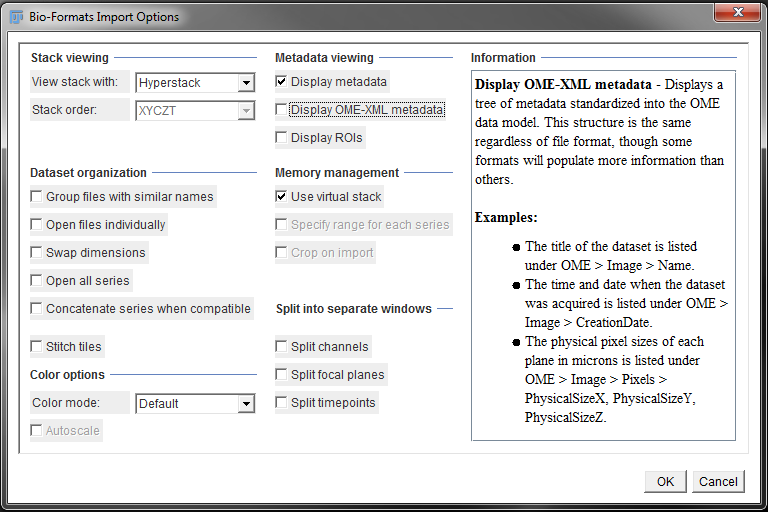
\includegraphics[width=0.8\textwidth]{mod1/figures/bioformats-import-dialog.png}%
		}
		\medskip
		\captionof{figure}{Bioformats Import Dialog.}\label{fig:bioformats-import-dialog}
		\end{center}
	\end{minipage}
	
	\item The next window allows you to select a series. Several microscope image formats are actually libraries of files. In this case, you should see three different files. Open one of the series.
	\item Two windows are opened. One showing the image, the other showing the metadata information. Scroll through the information and find the Dimension Length, Number of Elements and Unit. Use these values to calculate the pixel size.
\end{enumerate}

\end{taskbox}

\begin{taskbox}{Scale Bars}
Let's explore one final thing you usually have to include in your microscopy data: a scale bar that indicates the size of each pixel.

\begin{enumerate}
	\item Open the image sted-confocal.lif in /mod1/data by drag/drop or with \texttt{[Plugins > Bio-Formats > Bio-Formats Importer]}.  
	\item We now want to add a scale bar to our image. In this case, Fiji already knows the pixel size - let us check whether our previous calculations were correct. Go to \texttt{[Analyze > Set Scale...]}. This dialog should show you how many pixels are in one micrometer (Fig. \ref{fig:set-scale-dialog}).
	
	\begin{minipage}[t]{\linewidth}
		\begin{center}
		\adjustbox{valign=t}{%
			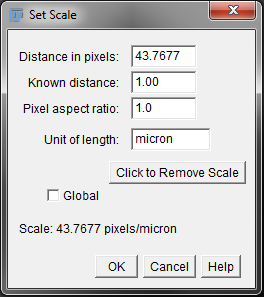
\includegraphics[width=0.4\textwidth]{mod1/figures/set-scale-dialog.png}%
		}
		\medskip
		\captionof{figure}{Set Scale Dialog.}\label{fig:set-scale-dialog}
		\end{center}
	\end{minipage}
	
	\item In case you have an image where information about the scale is visible in the image itself, you can then measure the length with a line and include this information in the dialog. Clicking on Global helps if you take one image of a micro-scale and want to use this information in other images you took with the same settings (e.g. on a small Lab-Microscope).
	\item Let's add a scale bar now. Use [Analyze > Tools > Scale Bar]. Similar to the calibration bar, the dialog lets you adjust various visual parameters (Fig. \ref{fig:scale-bar-dialog}).
	
	\begin{minipage}[t]{\linewidth}
		\begin{center}
		\adjustbox{valign=t}{%
			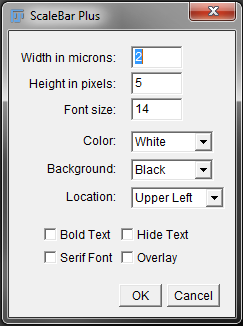
\includegraphics[width=0.4\textwidth]{mod1/figures/scale-bar-dialog.png}%
		}
		\medskip
		\captionof{figure}{Scalebar Dialog.}\label{fig:scale-bar-dialog}
		\end{center}
	\end{minipage}
	
\end{enumerate}

\end{taskbox}

\section{Figure publishing plugins for Fiji}
If you want to generate your figures completely in Fiji, there are great (published) plugins available that help you with this task (http://fiji.sc/2013-11-04\_-\_Plugins\_for\_making\_scientific\_Figures. as of 25/02/2015). The FigureJ plugin lets you specify a figure canvas on which you can place various images with labels and scale bars (http://imagejdocu.tudor.lu/doku.php?id=plugin:utilities:figurej:start, as of 25/02/2015).



% Module 2: Measuring intensities
\chapter{Measuring intensities}
An image contains one type of information: the intensities of the pixels in the image. In this chapter, we will show you how to work with this intensity information in a quantitative way. We will look at intensity distributions and how to perform measurements based on the intensity distributions in regions of the image (e.g. a cell). 

\section{Histograms}
Each pixel in an image has an intensity (a pixel value). The intensity histogram of an image is a plot that shows the distribution of pixel counts over a range of intensity values, typically the bit-depth of the image or the range between the minimum and maximum values within the image. The histogram can be used to examine the signal and background levels (useful when you want to identify objects of interest).

\begin{taskbox}{Working with histograms}
\begin{enumerate}
	\item Open the image hela-cells.tif in /mod2/data. This is another standard Fiji sample image showing HeLa cells. Lysosomes are red, mitochondria green and the nucleus blue. 
	\item We can show the histogram with \texttt{[Analyze > Histogram]}. The histogram is displayed in a new window (Fig. \ref{fig:histogram}). The x-axis shows the pixel value and the y-axis the count. Note that the histogram refers to the channel that was active when the command was called.
	
	\begin{minipage}[t]{\linewidth}
		\begin{center}
		\adjustbox{valign=t}{%
			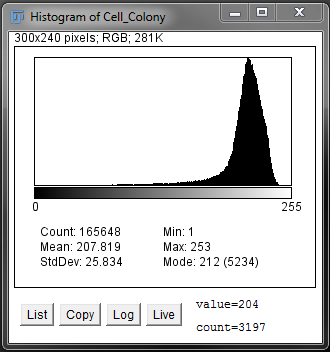
\includegraphics[width=0.4\textwidth]{mod2/figures/histogram.png}%
		}
		\medskip
		\captionof{figure}{Histogram.}\label{fig:histogram}
		\end{center}
	\end{minipage}
	
	\item Obtain the highest and lowest intensities from the histogram. What does the histogram range tell you?
	\item Click on [list] to obtain a list with values and counts. [Log] displays the same histogram on a log-scale.
	\item Click on [live] in the histogram dialog and change the channel. Observe the changes in the histogram and note the color changes in the depicted colormap bar.
	
\end{enumerate}

\end{taskbox}

\section{ROIs and the ROI Manager}
We now introduce a very powerful concept that is widely used for many types of analyses - the region of interest. Many operations can be applied to parts of the image when a region is selected by \emph{ROI} (region-of-interest) tools. The shape of the ROI is arbitrary; it can consist of a geometric shape, such as a circle or a line, but can be any selection of pixels. You already used ROIs when you selected a line or a point! Next, we will cover some basic ROI operations.

\begin{taskbox}{Working with ROIs}

One of the operations you can perform on a ROI is cropping:
\begin{enumerate}
	\item Open any image. Duplicate the image. Select a region by a rectangular ROI. Then, perform \texttt{[Image > Crop]} on the duplicate. Close the cropped image.
	\item Duplicate the original image again. Use the freehand selection to create a ROI on the duplicate. Crop the image. Note that the minimum and maximum values of your ROI have been used to determine a rectangular selection for the cropping.
\end{enumerate}

ROIs can be used to create image masks. An image masks is a binary image that define which parts of the image to analyze or measure.

\begin{enumerate}
	\item Open any image. Duplicate the image. Create a few circular ROIs (press <shift> during creation to keep multiple ROIs). 
	\item Use \texttt{[Edit > Clear Outside]} and then \texttt{[Edit > Fill]} to generate a mask image (this should look similar to fig. \ref{fig:binary-mask}. The 'Clear' command fills the respective area with the background color, 'fill' with the foreground color.
	
	\begin{minipage}[t]{\linewidth}
		\begin{center}
		\adjustbox{valign=t}{%
			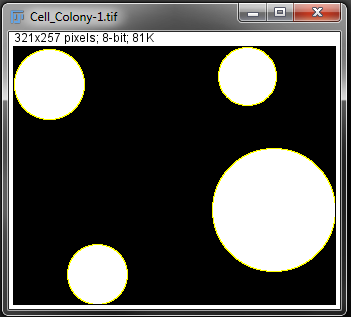
\includegraphics[width=0.4\textwidth]{mod2/figures/binary-mask.png}%
		}
		\medskip
		\captionof{figure}{Example binary mask.}\label{fig:binary-mask}
		\end{center}
	\end{minipage}
	
	\item Undo what you have done with \texttt{[Edit > Undo]}. You will notice that, in contrast to other programs, Fiji only allows to undo the most recent operation. This is done to minimize memory consumption. \texttt{[File > Revert]} allows you to go back to the last saved state.
	\item Go back to the original image. Use the command \texttt{[Edit > Selection > Create Mask]} to directly generate a mask image.
\end{enumerate}

Operations are usually performed on the selected ROIs and on the whole image if no selections exist. 
\begin{enumerate}
	\item Open any image. Duplicate the image. Select any ROI you like. 
	\item Observe that \texttt{[Edit > Invert]} only affects the selected pixels. Undo the inversion.
\end{enumerate}

Finally, there are several operations that work on a ROI itself without changing pixel values \texttt{[Edit > Selection > ...]}, see fig. \ref{fig:selection-options}. Let us explore a few of those options.

\begin{minipage}[t]{\linewidth}
		\begin{center}
		\adjustbox{valign=t}{%
			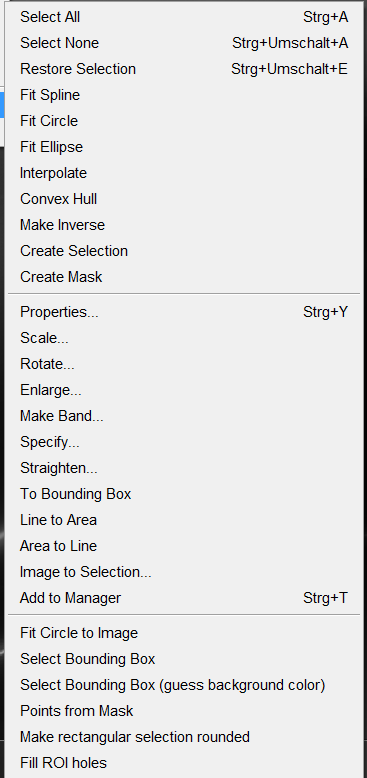
\includegraphics[width=0.4\textwidth]{mod2/figures/selection-options.png}%
		}
		\medskip
		\captionof{figure}{Selection options.}\label{fig:selection-options}
		\end{center}
	\end{minipage}


\begin{enumerate}
	\item Open an image, duplicate and draw a freehand selection with an outline that includes inner parts that are not selected. Fit a spline \texttt{[Fit Spline]}. This creates a smoothed version of the selection where individual points can now be dragged around and the shape can be changed. This can be useful to correct the outline of a shape (e.g. a worm or a cell). 
	\item Use \texttt{[To Bounding Box]}. This creates a rectangular region that just fits over the selection (this is the same as the crop area). Undo the last operation.
	\item Use \texttt{[Convex Hull]}. This creates an outline of the selection, where a straight line between every pair of points within the ROI is also within the ROI (Definition of a convex object in Euclidean space). This can be useful if you want to measure the extent of an object with an irregular shape. Undo the last operation.
	\item Explore the operations \texttt{[Scale]}, \texttt{[Make Inverse]}, \texttt{[Enlarge]} and \texttt{[Rotate]}.
	\item Each ROI has properties that can be displayed and changed with \texttt{[Properties]}. Especially useful when you work with multiple ROIs (and the ROI Manager, see below), can be ROI names (Fig. \ref{fig:roi-properties}). If you need the ROI coordinates outside Fiji, you can list the coordinates of the ROI as well.
	
	\begin{minipage}[t]{\linewidth}
		\begin{center}
		\adjustbox{valign=t}{%
			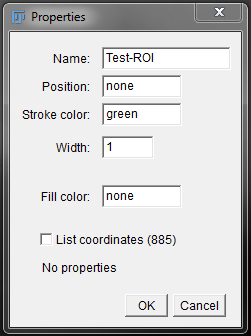
\includegraphics[width=0.4\textwidth]{mod2/figures/roi-properties.png}%
		}
		\medskip
		\captionof{figure}{ROI properties.}\label{fig:roi-properties}
		\end{center}
	\end{minipage}
	
\end{enumerate}

\end{taskbox}

\minisec{Managing multiple ROIs}
Fiji has an ROI manager to assist when you work with multiple ROIs. Open the ROI manager with \texttt{[Analyze > Tools > ROI Manager...]}. The manager allows you to add, delete and modify existing ROIs, save and load ROI coordinates, and change their display properties (Fig. \ref{fig:roi-manager}).

\begin{figure}[!ht]
	\begin{center}
		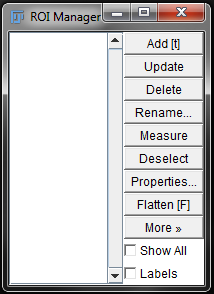
\includegraphics[width=0.3\textwidth]{mod2/figures/roi-manager.png}
		\caption{ROI manager.}\label{fig:roi-manager}
	\end{center}
\end{figure}

\begin{taskbox}{Working with the ROI Manager}
\begin{enumerate}
	\item Open the image hela-cells.tif in /mod2/data.
	\item Open the ROI Manager with \texttt{[Analyze > Tools > ROI Manager...]}.
	\item For the following analysis, we will only work on the bottom-most cell. Select the blue channel showing the nucleus. Use the ROI tools to create an accurate outline of the nucleus and add the selected region to the ROI manager. Rename the ROI to 'Nucleus'.
	\item Select the blue channel showing the mitochondria. In this channel, we can estimate the cell outline - create the outline and add the selected region to the ROI manager, rename ROI to 'Cell'.
	\item Let's say the task we want to solve is get the area of the cell, excluding the nucleus, for our further analysis. We now explore an option using the ROI manager, we will later explore another way using masks and image math. Select 'Nucleus' and 'Cell ROIs simultaneously. Then go to the [More>>] button and select the XOR operation. 
\emph{XOR} is the \emph{exclusive or} (exclusive disjunction). This is a logical operation that we apply to the ROIs. The XOR function returns the area where both inputs differ, i.e. not overlap. As the 'nucleus' ROI is located within the 'Cell' ROI, this subtracts the nucleus from the cell. Add the resulting ROI to the ROI Manager and rename to 'Cytoplasm'.
	\item Select all ROIs and save them on disk - we will use these ROIs for measurements. 
\end{enumerate}

\end{taskbox}

\section{Measurements}

The easiest way to read pixel values is moving the mouse pointer over individual pixels and reading their intensity value in the main Fiji bar. The histogram allows us to get the distribution of pixel intensities. Fiji has the function \texttt{[Analyze > Measure]} to obtain statistical information about pixel values within a ROI. \texttt{[Analyze > Set Measurements...] }allows us to select the parameters we want to measure. For example, following parameters can be obtained (Fig. \ref{fig:set_measurements-dialog}):
\begin{description}
	\item[Area] Area of selection in square pixels. If the image is calibrated, Area is displayed in according units.
	\item[Standard Deviation] Standard deviation of intensity values.
	\item[Min and Max Gray Value] Minimum and maximum intensities in selection.
	\item[Center of mass] Intensity-weighted spatial average.
	\item[Bounding rectangle] Bounding box, smallest rectangle enclosing selection.
	\item[Area fraction] The percentage of highlighted pixels, or the percentage of non-zero pixels.
	\item[Mean gray value] Mean intensity in selection.
	\item[Centroid] The average of all \emph{x} and \emph{y} coordinates in the selection.
	\item[Perimeter] The length of the outside boundary of the selection.
\end{description}

\begin{figure}[!ht]
	\begin{center}
		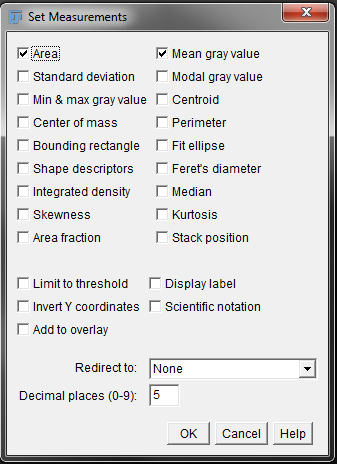
\includegraphics[width=0.4\textwidth]{mod2/figures/set-measurements-dialog.png}
		\caption{Set Measurements Dialog.}\label{fig:set-measurements-dialog}
	\end{center}
\end{figure}

\begin{taskbox}{Using the ROI Manager}
Now, we are going to combine ROIs (and the ROI Manager) with measurements -- you will see how powerful this already gets!
\begin{enumerate}
	\item Open the image hela-cells.tif in /mod2/data. Open the ROI Manager and load the previously generated ROI data.
	\item Measure the area and average intensity of the whole cell, the nucleus and the cytoplasm in the green channel and compare the results (Fig. \ref{fig:results-window}).
	
		\begin{minipage}[t]{\linewidth}
		\begin{center}
		\adjustbox{valign=t}{%
			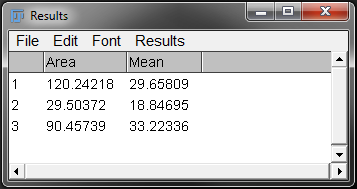
\includegraphics[width=0.3\textwidth]{mod2/figures/results-window.png}%
		}
		\medskip
		\captionof{figure}{Results window showing measurements.}\label{fig:results-window}
		\end{center}
	\end{minipage}
	
	\item Create a ROI in the background of the image (no cell), select the green channel and measure the average intensity again. Name the ROI 'Background' and update the saved ROI file; we will need this for further measurements.
\end{enumerate}	
\end{taskbox}

\section{Changing pixel intensities}
We now have seen various times that an image is represented as a matrix and that we can operate on individual pixels. In this section, we explore basic operations that allow us to modify the values of individual pixels in a ROI or the whole image. As you will see, you have to be careful with these operations, especially when you want to measure and/or compare intensities. However, they can be extremely useful to identify interesting regions of your images or enhance details.

\subsection{Arithmetic}
As an image is a matrix of numbers, we can do usual math on those pixels. We will go through one example where this might be useful and one example to show that things can go wrong if we are not careful.

\begin{taskbox}{Subtracting background levels}
A common task is the subtraction of the background levels of our images to make them comparable (background levels might vary). Subtracting a constant is the most basic background subtraction possible. 

\begin{enumerate}
	\item Open the image hela-cells.tif in /mod2/data. Open the ROI Manager and load the previously generated ROI data that includes the background ROI.
	\item Measure the average intensity in the background and note the value.
	\item Select the overall image \texttt{[Edit > Selection > Select All]} in the green channel. 
	\item Subtract the average background level from the green channel, using \texttt{[Process > Math > Subtract]}. You can also measure the backgrounds of the other color channels and subtract those as well.
\end{enumerate}

\end{taskbox}

\begin{taskbox}{Bit-depth/Format Problems}
A common task is the subtraction of the background levels of our images to make them comparable (background levels might vary). Subtracting a constant is the most basic background subtraction possible. 

\begin{enumerate}
	\item Open the image hela-cells.tif in /mod2/data. Duplicate the green channel.
	\item Look at the histogram of the green channel.
	\item Now, multiply the image by 2.5 - this increases the brightness of the image. 
	\item Generate the histogram again and compare the number of saturated values. As you can see, if the resulting value of a pixel is clipped if we get a value outside our bit-depth. If the result is a real number but our format only allows whole numbers, the resulting value would be rounded. Of course, this was a rather stupid example, but this is a common mistake when you perform more complicated calculations on your images.
	\item if you want, you can convert your image to an appropriate format and compare results.
	\item You can also try to perform the previous invert-example without the conversion to 32-bit.
	\end{enumerate}
	
\end{taskbox}

\subsection{Doing math with two images}
In the previous section, we operated with a single image and constant numeric values. Likewise, we can perform computations that involve two images. Assuming that both images have the same dimensions, we can perform calculations on each pair of pixels at the same position. For example, this type of operation can be used to subtract an image showing only (non-uniform) background from the image showing background + data or we can compare two images by obtaining their difference.

\begin{taskbox}{Background subtraction}
In this example, we are exploring a common method to subtract background information from a time-series. In the given example, we have moving bacteria that were imaged with phase contrast microscopy. The key idea for the background subtraction is that on each pixel, most of the time no bacteria is visible. We therefore create an average image and subtract this image from the original images to increase contrast of moving bacteria.

\begin{enumerate}
	\item Open the image bacteria-tracks.tif in /mod2/data. This image was create from supplementary video 1 of the publication: Rosser et al. (2013) Novel Methods for Analysing Bacterial Tracks Reveal Persistence in Rhodobacter sphaeroides, PLOS Computational Biology, DOI: 10.1371/journal.pcbi.1003276. Please note that this was not the original data, it seems that the supplementary movie was compressed!
	\item Perform a Z-projection to create an average image.
	\item Use \texttt{[Process > Image Calculator...]} to subtract the average image from each image in the original time-series and display the difference in a new window.
	\item Do you see any differences?
\end{enumerate}

Not surprisingly, the authors of the original publication used exactly this approach as the first step in their image processing.

\end{taskbox}

\begin{taskbox}{Math on Masks}
Before, we used the ROI Manager XOR function to obtain the cytoplasm ROI. We can obtain the same result using image masks and image calculations (actually this is likely happening behind the scenes anyway!).

\begin{enumerate}
	\item Open the image hela-cells.tif in /mod2/data. Open the ROI Manager and load the previously generated ROI data that includes the background ROI.
	\item Duplicate just the green channel.
	\item Select the Nucleus ROI and create a mask (look at the previous exercise if you forgot how to proceed). Duplicate the mask.
	\item Now, select the Cell ROI and create another mask.
	\item you should now have two image masks (black-and-white images, see fig. \ref{fig:image-masks}).	
	
		\begin{minipage}[t]{\linewidth}
		\begin{center}
		\adjustbox{valign=t}{%
			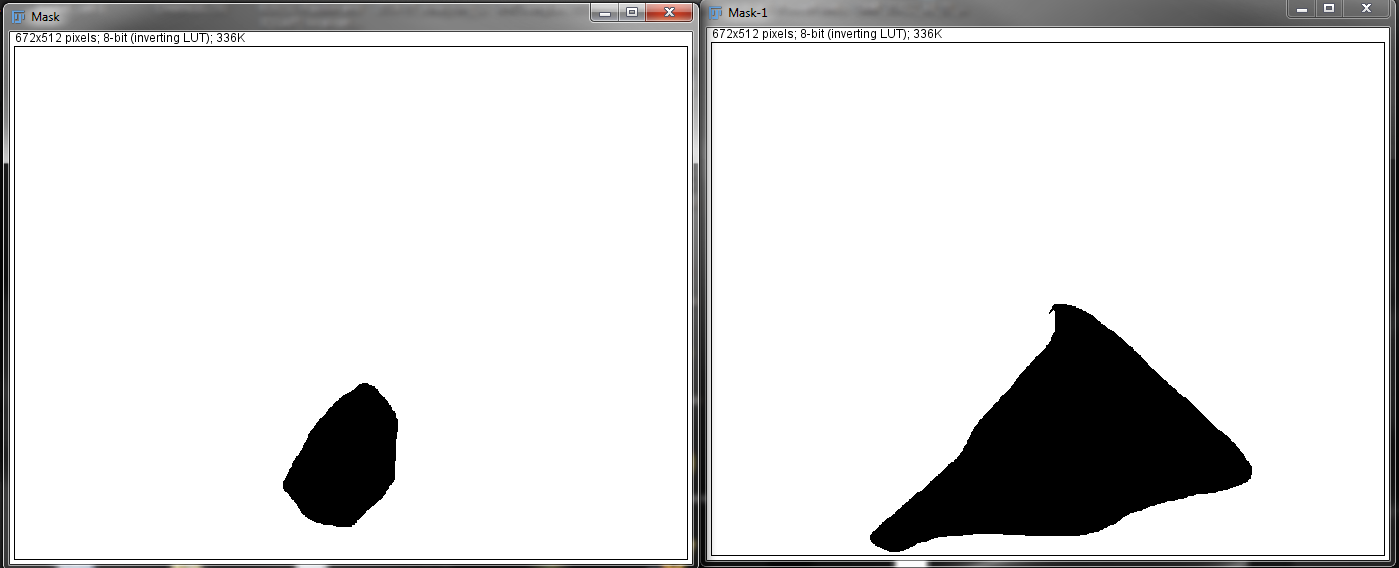
\includegraphics[width=0.8\textwidth]{mod2/figures/image-masks.png}%
		}
		\medskip
		\captionof{figure}{Image Masks.}\label{fig:image-masks}
		\end{center}
	\end{minipage}
	
	\item Calculate the XOR function using the binary data of both images (\texttt{[Process > Image Calculator...]}).
	\item Compare the results with the cytoplasm ROI.
	\item Using \texttt{[Edit > Create Selection]}, you can create a selection from the mask.
\end{enumerate}

\end{taskbox}

\section{Contrast enhancements}
You might already have experience with contrast enhancing of digital images, since most photo-editing software/apps have this function. Low contrast images have small differences in tones and objects are difficult to observe. If the contrast is too high, the tone difference is very high, the picture is 'over-exposed'. Contrast can be adjusted to optimize the appearance of the image. Contrast enhancement primarily changes the LUT, leaving the original data unaffected (it is affected if you apply the changes). Contrast enhancement should be used with care as pixel values are altered and intensity calculations become useless. Therefore, you should avoid contrast enhancements when you analyze intensities (this also applies to the figures that make your point!). Even if you treat all images the same way, you have to make sure that you avoid clipping and that results are not distorted by contrast enhancement.

\begin{taskbox}{Contrast Enhancement and Image Manipulation}
Let's assume you want to show gel data in your manuscript. After performing following steps, can you discuss why contrast enhancement might be considered fraud?
\begin{enumerate}
	\item Open the image gel.tif in mod2/data and duplicate the image (another Fiji sample image).
	\item Adjust Contrast and Brightness and compare images. What is the problem with the contrast-enhanced image (Fig. \ref{fig:contrast-problem})?
	
	\begin{minipage}[t]{\linewidth}
		\begin{center}
		\adjustbox{valign=t}{%
			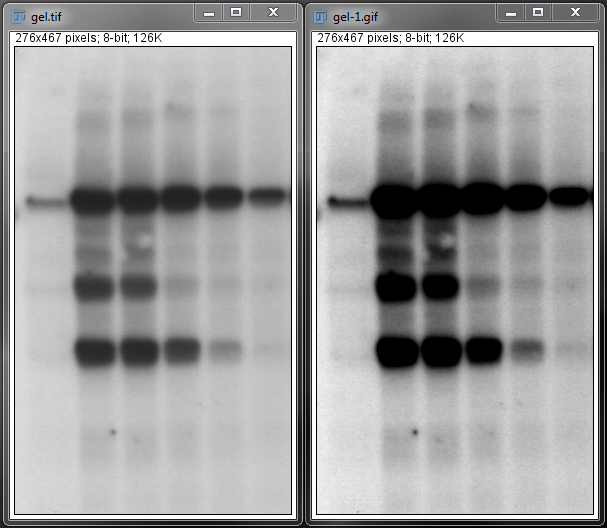
\includegraphics[width=0.8\textwidth]{mod2/figures/contrast-problem.png}%
		}
		\medskip
		\captionof{figure}{Contrast enhancement. The left gel plot shows the original data. Contrast enhancement in the right gel plot shows that you interpretation of this gel might be different.}\label{fig:contrast-problem}
		\end{center}
	\end{minipage}
	
	\end{enumerate}
\end{taskbox}

\subsection{Histogram Normalization}
With normalization, pixel values are normalized according to the minimum and the maximum pixel values in the image and bit-depth. If the minimum pixel value is \emph{pmin} and the maximum is \emph{pmax} in an 8-bit image, then normalization is done as follows:

\begin{equation*}
\mathit{NewPixelValue}=\frac{(\mathit{OriginalPixelValue}-\mathit{pmin})}{(\mathit{pmax}-\mathit{pmin})}\ast
255
\end{equation*}

\begin{taskbox}{Histogram Normalization}

\begin{enumerate}
	\item Open the image hela-cells.tif in /mod2/data and duplicate the green channel. Obtain a histogram.
	\item Use \texttt{[Process > Enhance Contrast]} on the duplicate. Set saturated pixels to 0, tick normalize and not equalize (Fig. \ref{fig:enhance-contrast-dialog}) and obtain a histogram afterwards.
	
	\begin{minipage}[t]{\linewidth}
		\begin{center}
		\adjustbox{valign=t}{%
			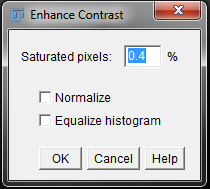
\includegraphics[width=0.3\textwidth]{mod2/figures/enhance-contrast-dialog.png}%
		}
		\medskip
		\captionof{figure}{Enhance Contrast Dialog.}\label{fig:enhance-contrast-dialog}
		\end{center}
	\end{minipage}
	
	\item Compare the histograms. 
	\item Leave the images open; you can also explore different settings.
	
	\end{enumerate}
\end{taskbox}

\subsection{Histogram Equalization}
Equalization converts pixel values so that the values are distributed evenly within the dynamic range. 

\begin{taskbox}{Histogram Equalization}

\begin{enumerate}
	\item Go to the original image showing the green channel.
	\item Use \texttt{[Process > Enhance Contrast]} on the duplicate. Set saturated pixels to 0, tick equalize, not normalize and obtain a histogram.
	\item Compare the histograms. 
	
	\end{enumerate}
\end{taskbox}

\subsection{Local Histogram Equalization}
Histogram equalization could also be performed on a local basis. This becomes powerful, as more local details could be contrast enhanced. In Fiji, you can use local histogram equalization with \texttt{[Process > Enhance Local Contrast (CLAHE)]}.

\section{Colocalization}



% Module 3: Measuring objects
\chapter{Working with objects - Generalized image analysis workflows}

In the module 'Measuring Intensities', you explored how you can manually define a region of interest and perform intensity measurements on this region. While this is already a commonly found approach, the manual labor can be very tedious or impossible with given resources. Another aspect that is often neglected is the possible (and likely) introduction of bias - outside actual clinical studies, a double blind approach is very uncommon. This module will present all components of a generalized image analysis workflow:

\begin{enumerate}
	\item Obtain raw image data. In this course, we assume that raw image data already exists and that this image data is suitable for the necessary analysis.
	\item Image visualization and preprocessing. This typically involves simple pixel operations and multiple image filters.
	\item Identify objects of interest (image segmentation). The preprocessed image is used to generate pixel label maps; in a simple case, this is based on a binary image (black = background, white = objects of interest).
	\item Manipulate objects. The detected objects are modified and enhanced. For example, this can involve cleaning object boundaries, removing holes, splitting or merging objects.
	\item Perform measurements. In the last step, you convert the finally identified objects into numbers for further (statistical) analysis. For example, the derived numbers can be based on intensity, shape, texture or object relationships.
\end{enumerate}

\section{Image preprocessing}

We now generalize this concept of pixel operations by looking at an image as a discrete function. For a 2D image, $f(x,y)$ maps from $R^2$ to $R$, giving the intensity at position $(x,y)$. In this view, any pixel operation $o$ can be expressed as $g\left(x,y\right)=o\left(f\left(x,y\right)\right)$, where $g(x,y)$ is the modified image. The operations we already know are either simple arithmetic- or histogram-based methods. 

Another type of very powerful operations is the \emph{image filter}. Often, image preprocessing involves the (sequential) application of various image filters. Image filters are local operations where the \emph{neighborhood} (surrounding pixels) of each pixel determines the new intensity value. The pixel neighborhood is also called the \emph{kernel}. These filters are mainly used to smooth the image (suppress high frequencies) or enhance edges (suppress low frequencies).

Image filters can be performed on the spatial domain (the image you know with x/y/z axes) or on the frequency domain (Fourier transformed image). For simplicity, we completely skip the Fourier transform, frequency domain filtering and the mathematical reasoning why it can make sense to transform an image into the frequency domain, perform (linear) filtering, and transform the image back to the spatial domain. Furthermore, we will restrict our explanations and examples to 2 dimensional (discrete) images. 

\subsection{Convolution, Correlation \& Kernels}

Convolution is the mathematical operation behind many of the image filters we will discuss. As described, the basic idea is that a neighborhood of pixels, a window with finite size and shape, is placed on top of each pixel and that the new pixel value is determined by the weighted sum of all pixels within this neighborhood. This window with the weights is called the \emph{kernel}. 

Again, we look at the image as a matrix of pixels and do the same for the kernel, the neighborhood with the weights. We then perform the weighted sum of all pixels within the kernel and repeat for every pixel in our image (Fig. \ref{fig:convolution-example}).

\begin{figure}[!ht]
	\centering
		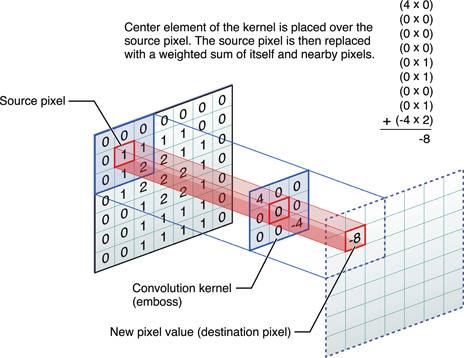
\includegraphics[width=0.70\textwidth]{mod3/figures/convolution-example.png}
	\caption{Convolution example. A single location of a 2D convolution is shown. The image was taken from \cite{MacDev2011}}
	\label{fig:convolution-example}
\end{figure}

If we want to convolve a pixel at position $(x,y)$ of an image $F$ with the rectangular kernel $K$, centered around $(x,y)$, with width $\omega$, we can write:
\[
	\left[F\ast K\right]\left(x,y\right)=\sum_{i=-\omega}^{i=\omega}\sum_{j=-\omega}^{j=\omega}K\left(i,j\right)\cdot F\left(x-i,y-j\right)
\]

For better illustration, let us perform the convolution on a small example, we average an image showing a vertical white line on black background with a 3x3 smoothing kernel (this operation is explained below):
\[
	\begin{array}{|c|c|c|c|c|}
	\hline
	0&0&255&0&0\\
\hline
0&0&255&0&0\\
\hline
0&0&255&0&0\\
\hline
0&0&255&0&0\\
\hline
0&0&255&0&0\\
\hline
	\end{array} 
	\ast 
	\begin{array}{|c|c|c|}
	\hline
	1/9&1/9&1/9\\
\hline
1/9&1/9&1/9\\
\hline
1/9&1/9&1/9\\
\hline
	\end{array}
	=
	\begin{array}{|c|c|c|c|c|}
	\hline
	0&57&57&57&0\\
\hline
0&85&85&85&0\\
\hline
0&85&85&85&0\\
\hline
0&85&85&85&0\\
\hline
0&57&57&57&0\\
\hline
	\end{array} 
\]

Figure \ref{fig:convolution-demo} looks at a few steps of the convolution to illustrate how the resulting image is calculated.

\begin{figure}[!ht]
	\centering
		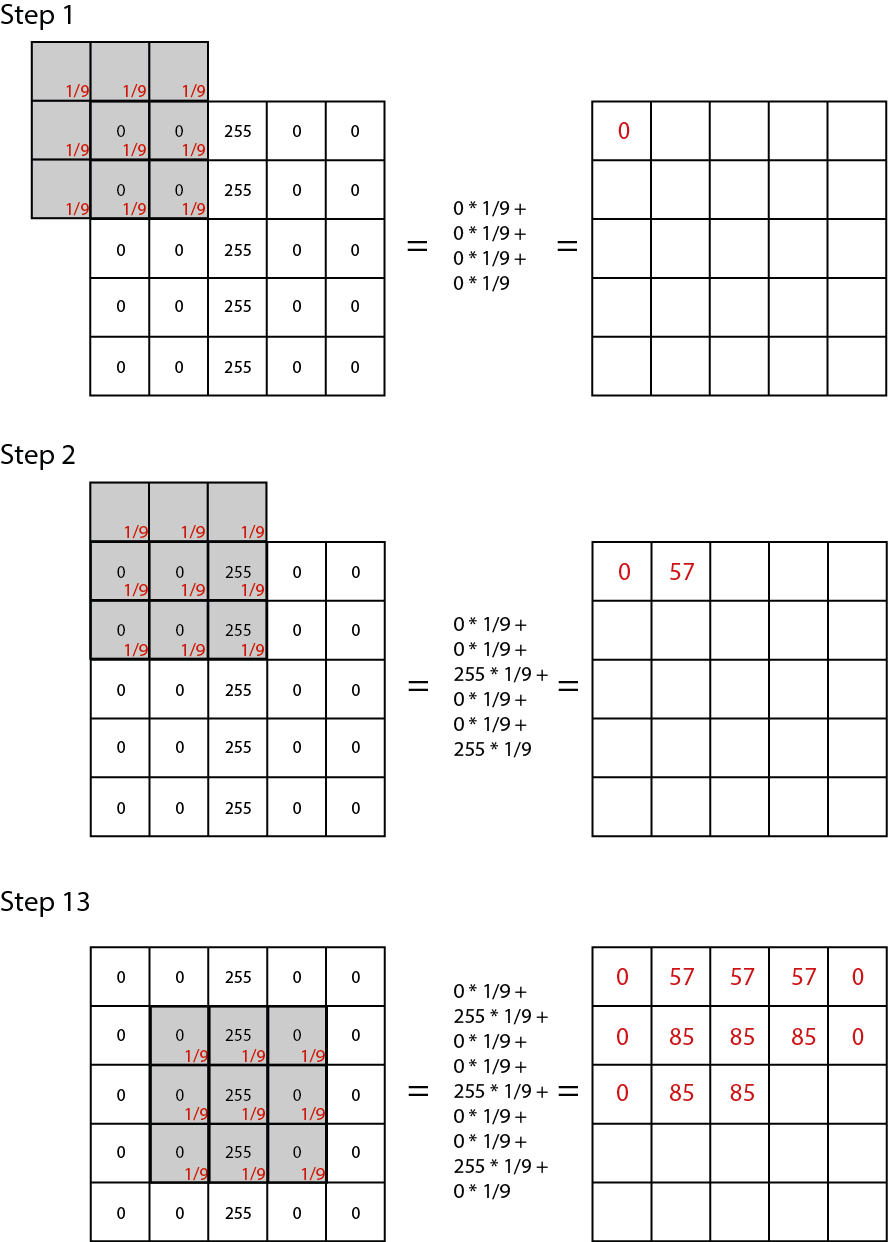
\includegraphics[width=0.60\textwidth]{mod3/figures/convolution-demo.png}
	\caption{Example steps of the convolution}
	\label{fig:convolution-demo}
\end{figure}

\newpage
\begin{taskbox}{Working with Image Filters}
Let us compare the previous example with the operation performed in Fiji.

\begin{enumerate}
	\item Generate an 8-bit, 5x5 pixel black image with a white vertical line as shown in the convolution example. Duplicate and zoom in to observe individual pixels and check whether the intensity values of the black pixels are zero and the values of the white pixels are 255.
	\item Go to \texttt{[Process > Filters > Convolve...]}. Change the default kernel in the Convolver dialog to (Fig. \ref{fig:convolver-dialog}): 
	\[
		\begin{array}{|c|c|c|}
	\hline
	1&1&1\\
\hline
1&1&1\\
\hline
1&1&1\\
\hline
	\end{array}
\]
	Note that we did not enter 1/9; the values are automatically divided by the number of elements in the kernel if 'Normalize Kernel' is ticked. Select 'Preview' if you directly want to observe the effects of your chosen kernel.
	
	\begin{minipage}[t]{\linewidth}
		\begin{center}
		\adjustbox{valign=t}{%
			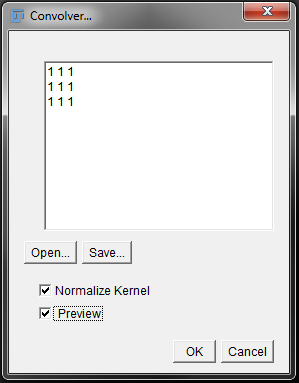
\includegraphics[width=0.3\textwidth]{mod3/figures/convolver-dialog.png}%
		}
		\medskip
		\captionof{figure}{Convolver Dialog.}\label{fig:convolver-dialog}
		\end{center}
	\end{minipage}
	
	\item Compare the new pixel values with the values shown in the example. Do you observe any differences? You should note that pixels at the border of the image can show differences. This is caused by a different way to treat image borders. While the example simply ignores kernel positions outside the image, Fiji increases the image size to fit the kernel within the image (padding). These extra pixels are duplicates of border pixels and therefore, the results differ.
	
	\end{enumerate}
\end{taskbox}

\minisec{Convolution and Correlation}

A convolution is a correlation with the kernel rotated by 180 degrees. This makes no difference if the filter is symmetric (e.g. Gaussian). The reflection of the kernel has a few important effects. One is that the convolution is associative ($f * g * h = f * (g * h)$) while the correlation is not; i.e. the associativity allows you to pre-convolve several filters into a single filter that gets applied to your image. The correlation describes the comparison between the kernel and the pixel neighborhood and is, for example, used in template matching as associativity is not important for this task. Also, the convolution is a multiplication in the frequency domain and it can be faster to perform the filtering in the frequency domain (depending on image and kernel size). 

\begin{taskbox}{The point spread function (PSF)}

The image you obtain with a microscope is blurred by the optics of the microscope itself. The point spread  function describes the impulse response of the microscope, i.e. the 3D diffraction pattern resulting from a single point. In microscopes (non-coherent systems), the image formation process is linear, which means that the imaging of many objects produces a result that is the sum of individually imaged objects. Therefore, image formation in a microscope can be seen as a convolution of the true object with the PSF. Estimating the PSF of a microscope then allows image deconvolution -- a process where the true image is estimated by trying to reverse the effects of the convolution. The problem is that deconvolution is an ill-posed problem -- no solution, or no unique solution might exist and noise can strongly influence a solution. Computing intense deconvolution algorithms are used to approximate the true image; a PSF for deconvolution can be obtained by measuring sub-resolution beads with know radii or by theoretical estimation using parameters of the optical system. 

In this exercise, we use an artificial ground-truth image and convolve this image with a single slice of a cropped and low bit-depth version of a measured PSF. 

\begin{enumerate}
	\item Open the images artificial-groundtruth.tif and PSF-LeicaSP8-63x-Ar488.tif in /mod3/data. The image shows a cropped, 8 bit, x/y slice through a 3D PSF taken at the center (focal plane). 
	\item Convolve the groundtruth image with the PSF by loading the file PSF-LeicaSP8-63x-Ar488.txt in the convolver dialog.
	\item Compare the groundtruth image with the convolved image. This is what happens every time you take an image with the microscope! (Although this is only a 2D, simplified example).
	\end{enumerate}
\end{taskbox}

\subsection{Linear Filters}
Convolution is the mathematical operation behind linear filters; and in the following, we will look at some of the most common linear filters available.

\subsubsection{Averaging filter}
An averaging operation (also called smoothing, arithmetic mean or box-car filter) is used to suppress noise in an image. The size of the structures that are suppressed is dependent of the kernel size. Small fluorescence fluctuations will be suppressed by a small filter; increasing the filter size, larger structures will be reduced in size and smoothed into the surrounding regions. Manually varying the filter size allows you to decide the optimal scale of the smoothing for your analysis.

This filter was already shown in the convolution demonstration and the first exercise, the kernel (without normalization to the number of elements) is:
	\[
		\begin{array}{|c|c|c|}
	\hline
	1&1&1\\
\hline
1&1&1\\
\hline
1&1&1\\
\hline
	\end{array}
\]

\begin{taskbox}{Averaging images}

\begin{enumerate}
	\item Open the image microtubuli.tif in /mod3/data. Zoom into the image and observe the fluorescence fluctuations along the microtubuli.
	\item Preview the smoothing filter with a kernel size of 3x3 (see above), using \texttt{[Process > Filters > Convolve...]}. Then increase the kernel size to 5x5 and 7x7 and compare the results (duplicate the images!). What happens when the size of the kernel becomes larger? Can you enter a kernel size of 2x2?
	\item The averaging filter has its own direct command in Fiji. Go to \texttt{[Process > Filters > Mean...]}. You can choose a radius and optional preview in the next window. A radius can be given instead of size in X and Y as the kernel mask is circular -- the neighborhood can be defined arbitrarily! Circular kernels are common as pixels the outermost pixels have the same distance to the pixel of interest (Circular kernels can be shown with \texttt{[Process > Filters > Show Circular Masks...]}). Try different radii to obtain the best smoothing to suppress small fluorescence fluctuations.
	\item To show the effect of the filter more directly, you can subtract the smoothed from the original image.
	\end{enumerate}
\end{taskbox}

\subsection{Gradient filters}

Image features with high spatial frequencies (edges) are those where intensity varies greatly over short image distances (e.g. neighboring pixels). These changes over distance can be seen as a derivative (like velocity is the derivative of position over time). For our images, we use the \emph{gradient} as a generalization of the derivative of a function in one dimension (like velocity), to a function in several dimensions (like our 2D images). For our 2D images $I(x,y)$, we can write the gradient as:
\[
	\nabla I(x,y)=\left(\frac{\delta I}{\delta x},\frac{\delta I}{\delta y}\right)
\]

A common use for gradient filters is edge detection. A large gradient value of a pixel might indicate an edge and edges could then be traced along those pixels (perpendicular to gradient direction). For example, edge detection can be very useful if your structures of interest vary in absolute intensity but are always distinctive against their direct surroundings. 

\minisec{Find Edge (Sobel Filter)}
The find edge filter is used to create an image which emphasizes edges. It uses an approximation of the gradient to create two 3x3 kernels which are convolved with the original image $I$ (kernels are an approximation of the derivative in horizontal, respective vertical direction) to create two output images $J_{x}, J_{y}$:
	\[
		J_{x}=\left[\begin{array}{ccc}
	1&0&-1\\
2&0&-2\\
1&0&-1\\
	\end{array}\right]\ast I, J_{y}=\left[\begin{array}{ccc}
	1&2&1\\
0&0&0\\
-1&-2&-1\\
	\end{array}\right]\ast I
\]

The gradient magnitude image $J$ is then calculated with:
\[
	J=\sqrt{J_{x}^{2}+J_{y}^{2}}
\]

\minisec{Sharpen (Laplacian Filter)}

The sharpen filter is also often used to emphasize changes in pixel intensities. In this case, the 3x3 kernel is approximated by the sum of the second derivatives:
	\[
		\begin{array}{|c|c|c|}
	\hline
	-1&-1&-1\\
\hline
-1&12&-1\\
\hline
-1&-1&-1\\
\hline
	\end{array}
\]

\begin{taskbox}{Gradient Filters}
\begin{enumerate}
	\item Open the image microtubuli.tif in /mod3/data. Zoom into the image and observe the fluorescence fluctuations along the microtubuli. Remember to duplicate the images before testing any processing.
	\item At first, test the sharpen filter with \texttt{[Process > Sharpen]} and optionally using the kernel in the convolution dialog.
	\item The find edge filter can be tested directly using \texttt{[Process > Find Edges]}. If you want to explore the filter a bit more, you can also generate both filtered images, convert those to 32 bit and perform the calculations by yourself. Are the results identical?
	\item What happens to the noise if you use the sharpen filter? 
	\item What happens if you first use a smoothing filter and then the edge detection filter?
	\end{enumerate}
\end{taskbox}

\subsubsection{Gaussian filters}

A very important linear filter that smooths an image and reduces noise is the \emph{gaussian filter}. In difference to the mean filter, pixels in the neighborhood are weighted with their distance to the pixel of interest. The weights are obtained by a gaussian function where the width $\sigma$ of the gaussian function $g(x,y)$determines the kernel size. $A$ is a scaling factor used for normalization:
\[
	g(x,y)=A e^{\left(\frac{x^2+y^2}{2\sigma^2}\right)}
\]

If you want to smooth your image, it is always a good idea to not only explore the averaging filter but also the gaussian filter. Again, varying $\sigma$, you can determine the optimal filter size for your application.

\minisec{Difference of Gaussian filter (DoG)}
Let's say you want to suppress small structures but also large structures and focus on detecting structures within a certain size range. In this case, you could combine two gaussian filters: one with a small $\sigma$ to suppress small structures and one with a large $\sigma$ to suppress large structures as well. When you then subtract the second filtered image from the first filtered image, the image that is left contains information between both smoothing scales. 

\begin{taskbox}{Gaussian Filters}
\begin{enumerate}
	\item Open the image microtubuli.tif in /mod3/data. Zoom into the image and observe the fluorescence fluctuations along the microtubuli. Remember to duplicate the images before testing any processing.
	\item The gaussian filter can be tested using \texttt{[Process > Filters > Gaussian Blur...]}. 
	\item Try to find an optimal value for $\sigma$.
	\item Implement a DoG filter with $\sigma$ values of $1$ and $10$.
	\end{enumerate}
\end{taskbox}

\begin{taskbox}{Unsharp Mask Filter}
Let's illustrate the power of combining filters and image math with another example. In this case, we will replicate the unsharp mask filter. This is a very common filter available in many software packages, e.g. for photo editing, but has to be used very carefully for quantitative scientific analysis.

\begin{enumerate}
	\item Open the image microtubuli.tif in /mod3/data. Duplicate.
	\item Use a gaussian filter with a $\sigma$ of $2$. 
	\item Multiply the gaussian filtered image with a weight $w$ of $0.8$.
	\item Subtract the weighted image from the original image.
	\item Divide the resulting image by $0.2$. 
	\item Last, compare your results to the results of \texttt{[Process > Filters > Unsharp Mask...]}.
	\end{enumerate}
\end{taskbox}

\subsection{Nonlinear Filters}
In addition to linear filters which can be implemented with a convolution, we can also use nonlinear filters to enhance our images. We will discuss one particular class of such filters (rank filters), focusing on the median filter. This filter or its variants can be very powerful when you want to remove noise but maintain other details of the image or you want to be less susceptible to outliers. 

\minisec{Median, maximum and minimum filters}
For the median, maximum and minimum filters, pixels in the neighborhood are sampled and then sorted by their intensity values. Let's assume you have an 3x3 image part surrounding the pixel with value 100, such as:
	\[
		\begin{array}{|c|c|c|}
	\hline
	0&95&105\\
\hline
0&100&110\\
\hline
0&0&90\\
\hline
	\end{array}
\]
 The sorted list would look like: $0,0,0,0,90,95,100,105,110$. The median filter would update the pixel value from 100 to 90. The mean filter would update to a value of 56. If this pixel is part of an edge, the median filter would be better to maintain this edge. The maximum and minimum filters use the same sorted list but update the pixel with either the highest or the lowest value.

\begin{taskbox}{Median Filter}
\begin{enumerate}
	\item Open the image microtubuli.tif in /mod3/data. Before we do any further processing, we add some Salt-and-Pepper noise using \texttt{[Process > Noise > Salt and Pepper]}. This sets random pixels to the lowest or highest values.
	\item Duplicate the image with added noise and perform the mean filter to suppress the just added noise (find a suitable radius).
	\item Now, use the median filter \texttt{[Process > Filters > Median]} with the same radius.
	\item Which filter works better?
	\end{enumerate}
\end{taskbox}

\begin{taskbox}{Background subtraction and batch processing}
To make this exercise more interesting, we first establish the method we want to use and then apply it to many files automatically. If a certain task is performed multiple times, it is called \emph{batch processing}. 

\begin{enumerate}
	\item Open the image xu2015-adipocytes.tif in /mod3/data. This image was provided as an example image by Elaine Xu (March 2015, Bruening lab, MPI Stoffwechselforschung). The image shows adipocytes and is a good example to illustrate uneven illumination and how to improve the image with background subtraction.
	\item At first, we explore a method to subtract the background. For this, we first perform a Gaussian blur on a duplicate image with a large $\sigma$ of $20$. This creates a very blurry image that already shows that we picked up the uneven illumination. You can look at a line profile in the original and the blurred image.
	\item Now we subtract the original image from the blurred image. Adjust brightness/contrast to confirm that background was subtracted. As the gaussian blur is a lowpass-filter, the subtraction of this lowpass image can be considered as a (pseudo) highpass filtering.
	\item Fortunately, Fiji already has a function embedded that performs a similar operation for background subtraction, called a rolling ball background subtraction (Same idea: somehow calculate an average for every pixel. However, the actual calculations differ). 
	\item We now want to perform the background subtraction on all image files in a certain folder. For this, we \emph{record} our actions and then use the recorded sequence on each of those files.
	\item Close all images except the original xu2015-adipocytes.tif.
	\item To start the recording, perform \texttt{[Plugins > Macros > Record...]}. A Recorder window pops up (Fig. \ref{fig:recorder-dialog}). Make sure that 'Macro' is selected in Record and nothing else.
	
	\begin{minipage}[t]{\linewidth}
		\begin{center}
		\adjustbox{valign=t}{%
			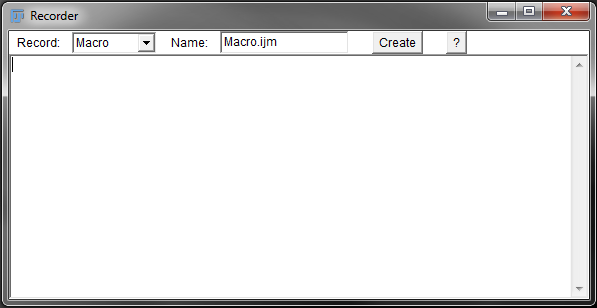
\includegraphics[width=0.8\textwidth]{mod3/figures/recorder-dialog.png}%
		}
		\medskip
		\captionof{figure}{Recorder window.}\label{fig:recorder-dialog}
		\end{center}
	\end{minipage}
	
	\item Do \texttt{[Process > Subtract Background...]}, set the rolling ball radius to $20$ (Fig. \ref{fig:rollingball-dialog}). After you clicked on 'ok', the operation gets performed and the recorder should show following line: \texttt{run("Subtract Background...", "rolling=20");}. 
	
	\begin{minipage}[t]{\linewidth}
		\begin{center}
		\adjustbox{valign=t}{%
			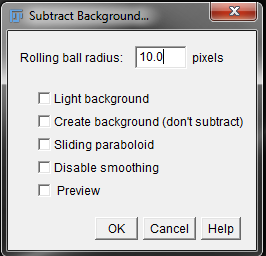
\includegraphics[width=0.3\textwidth]{mod3/figures/rollingball-dialog.png}%
		}
		\medskip
		\captionof{figure}{Subtract background window.}\label{fig:rollingball-dialog}
		\end{center}
	\end{minipage}
	
	\item Select the line and copy (Strg+C). Go to \texttt{[Process > Batch > Macro...]}. In the batch processing window, select the input folder /batch-files in /mod3/data. This folder contains 5 identical adipocyte images with different names. Also, choose an output folder, make sure that this output folder exists. Paste the line of code into the window (Fig. \ref{fig:batch-process-dialog}). and click on 'Process'. Check the chosen output folder for the results. 
	
		\begin{minipage}[t]{\linewidth}
		\begin{center}
		\adjustbox{valign=t}{%
			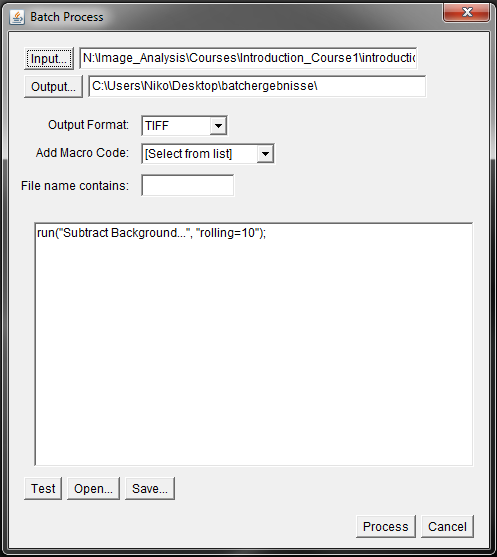
\includegraphics[width=0.8\textwidth]{mod3/figures/batch-process-dialog.png}%
		}
		\medskip
		\captionof{figure}{Subtract background window.}\label{fig:batch-process-dialog}
		\end{center}
	\end{minipage}
	
	\end{enumerate}
\end{taskbox}

When you try to perform a batch processing where a function requires explicit file names the batch processor will fail because it does not know that these need to be replaced (e.g. when the sequence Duplicate Image, Gaussian, Image Calculator is used). In this case, we have to create a macro where individual file names get replaced. Unfortunately, this requires a little bit of very basic understanding of programming principles (we need variables, for-loop and a function). As this is outside the scope of this module, we will not discuss those concepts (however, they are important for more complex automated workflows). 

\section{Image segmentation}

Image segmentation is a process where every pixel in an image obtains a label, such that pixels with the same label share characteristics. Typically, this is done to detect \emph{objects} or structures of interest. Sometimes, these objects are called \emph{connected components}. Basically, this is what you have already done using regions of interest to mark the pixels belonging to a nucleus or cytoplasm. This can be called manual segmentation and works if there is not too much data to analyze. Overall, it is preferable to automate the process of segmentation; not only because it is faster, but also because it should lead to better reproducibility and lower bias of the results. 

\subsection{Thresholding}

A very simple and easy to understand image segmentation method is called \emph{thresholding}. In this method, each pixel belongs to one of two groups: background or foreground (black or white, object or not object). For images obtained with fluorescence microscopy, this is easy to understand: we typically have dark background with light objects. Thresholding image $f\left(x,y\right)$ with a thresholt $T$ then leads to extraction of the objects in image $g\left(x,y\right)$:
	\[
		g\left(x,y\right)=\begin{cases}
		1 &\text{if } f\left(x,y\right)>T\\
		0 &\text{otherwise}
			\end{cases}
\]

Image $g\left(x,y\right)$ is a binary image, only consisting of black and white pixels.

\begin{taskbox}{Thresholding with contrast adjustment}
Let us first have a look at the effects of thresholding using brightness/contrast adjustments.

\begin{enumerate}
	\item Open the image cell-colony.tif in /mod3/data. Open the brightness/contrast adjustment window. Observe the slope of the line that shows the change in (displayed) intensity between the minimum and maximum pixel values in the histogram (Fig. \ref{fig:bc-window}, red line).
	
	\begin{minipage}[t]{\linewidth}
		\begin{center}
		\adjustbox{valign=t}{%
			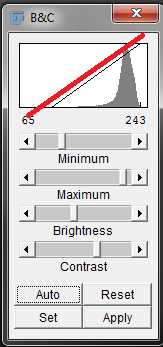
\includegraphics[width=0.3\textwidth]{mod3/figures/bc-window1.png}%
		}
		\medskip
		\captionof{figure}{Brightness and Contrast adjustment.}\label{fig:bc-window}
		\end{center}
	\end{minipage}
	
	\item Now, set the contrast to the maximum value and observe that the slope of the line changes until the line appears nearly vertical. The image is a black and white image now, everything to the left of the line is black, everything right of the line is white (the majority of the pixels as seen in the histogram).
	\item If you now change the brightness, you can move this vertical line around and observe that the number of pixels identified as white (black) changes.
	\end{enumerate}
\end{taskbox}

\begin{taskbox}{Manual thresholding}
Instead of adjusting the contrast, Fiji has a specialized function to adjust the threshold \texttt{[Image > Adjust > Threshold...]}.

\begin{enumerate}
	\item Open the image cell-colony.tif in /mod3/data if it is not already open. 
	\item Do \texttt{[Image > Adjust > Threshold...]} to open the threshold adjustment window (Fig. \ref{fig:adjust-threshold-dialog}). In this window, you can set the intensity for the threshold. Furthermore, you can select whether you have a dark or light background to determine whether you are interested in light or dark objects. Note that you can select a window for your threshold, by setting the lower and upper values to a value outside the extremes. This is called a \emph{density slice} and can be used to detect objects that fall within a certain intensity range.
	
	\begin{minipage}[t]{\linewidth}
		\begin{center}
		\adjustbox{valign=t}{%
			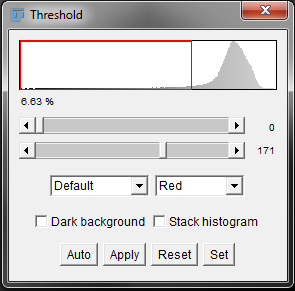
\includegraphics[width=0.4\textwidth]{mod3/figures/adjust-threshold-dialog.png}%
		}
		\medskip
		\captionof{figure}{Adjust threshold window.}\label{fig:adjust-threshold-dialog}
		\end{center}
	\end{minipage}
	
	\item Change values and play with different settings until you think you found an optimal threshold. How difficult is it to obtain an optimal threshold, i.e. how sensitive is the result to your chosen value?
	\end{enumerate}
\end{taskbox}

Manually thresholding an image is already a powerful way to detect objects of interest. But what should you do if you cannot apply the same threshold value for all images you want to analyze? Of course you could manually choose a value for each image. However, this can introduce a bias into your results. A better option would be to automatically determine the optimal threshold value for each image, using the same algorithm. Fiji already has a variety of algorithms that you can choose from (Fig. \ref{fig:all-thresholds}):

\begin{itemize}
	\item Huang
	\item Intermodes
	\item IsoData
	\item Li
	\item MaxEntropy
	\item Mean
	\item MinError
	\item Minimum
	\item Moments
	\item Otsu
	\item Percentile
	\item RenyiEntropy
	\item Shanbag
	\item Triangle
	\item Yen
\end{itemize}

\begin{figure}[!ht]
	\centering
		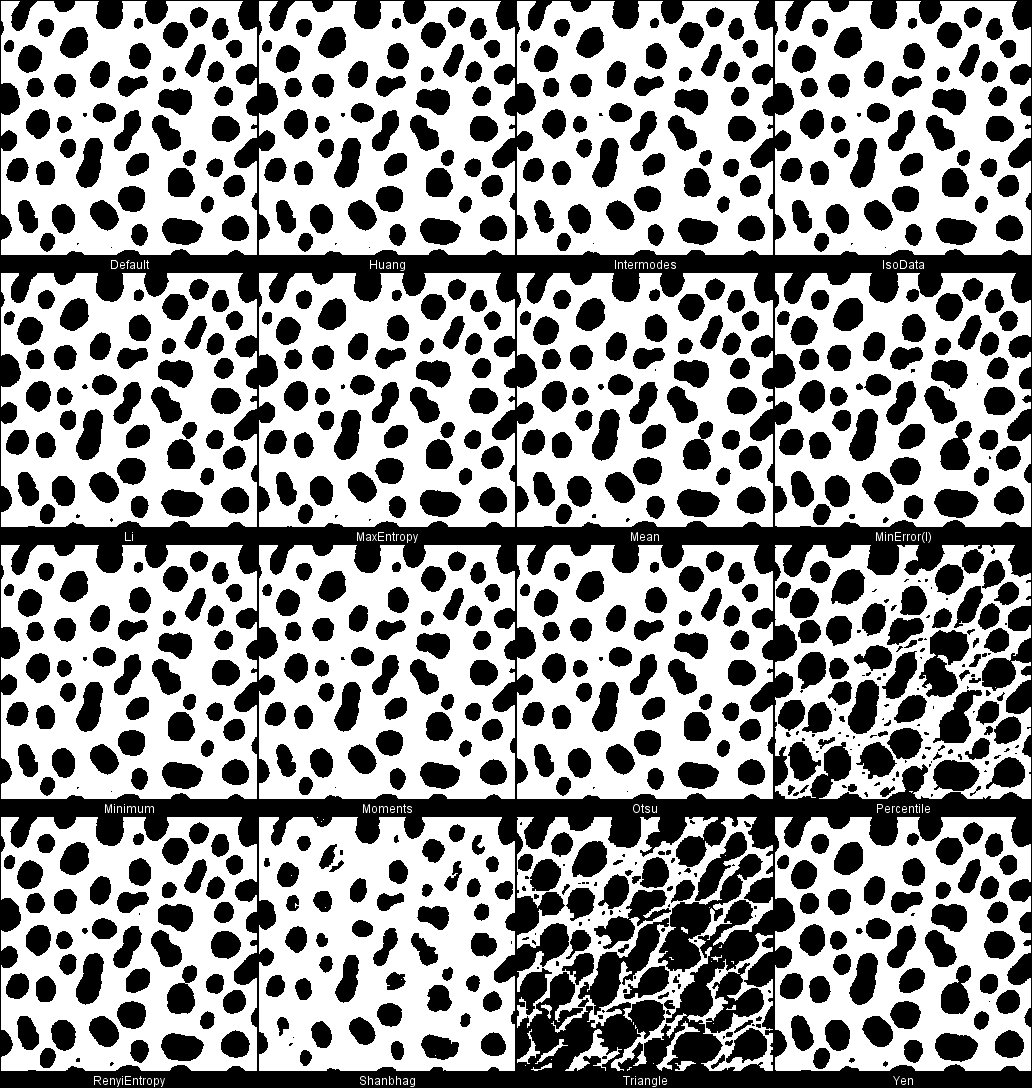
\includegraphics[width=0.80\textwidth]{mod3/figures/all-thresholds.png}
	\caption{Results of all available thresholding methods, using [Image > Adjust > Auto Threshold], Try All. }
	\label{fig:all-thresholds}
\end{figure}

Choosing an algorithm can theoretically be done by looking at the details of the algorithm and determining best which method suits your data. In practice, however, you can simply try all and choose the one that suits your purposes best. 

Let us have a look at one of the thresholding methods, \emph{ Otsu's method}. This algorithm makes the assumption that two classes of pixels are in an image, with each class having a distribution of intensity values. The algorithm calculates the optimum threshold that separates these two classes so that the variance of pixels within each class is minimal. This algorithm is very common, easy to understand and implement. 

\begin{taskbox}{Automated thresholding}
\begin{enumerate}
	\item Open the image hela-cells.tif in /mod3/data. In this task, we first want to automatically identify the nuclei. Select the appropriate channel and duplicate. 
	\item Test all available thresholding methods. You can see that most method already produce very nice results.
	\item In the next step, we want to identify the lysosomes (red). Try to threshold the appropriate channel with Otsu's method. Are the results good enough?
	\item As you can see, the algorithm already works relatively well, but is not good enough for our purposes. Can you think of a reason why the method fails in some parts of the cells? 
	\item After an analysis, we come to the conclusion that background signal is too high in parts of the cell. Therefore, we now first use a background subtraction (e.g. with a rolling ball radius of 10 pixels) before we threshold with Otsu's method. Do the results improve?
	\item Finally,try to use the green channel to identify the cells' cytoplasm. Again, it seems that an image filter might improve the results. Try a gaussian filter with varying sigma values to improve the results. At the end, the result we obtain is not perfect but might be sufficient for our needs. You will see in section about binary images how we could still improve on this thresholding. 
	\end{enumerate}
\end{taskbox}

\subsection{Binary Images}
Thresholding into two pixel classes leads to a binary image. In this section, we will learn how operations on binary images can be used to process an image to facilitate further analysis. 

\subsubsection{Morphological operations}
Morphological operations are very similar to image filters, only that in this case, logical operations are performed on the image. Similar to image filters, a small \emph{structuring element} (kernel in image filters) is moved over the image pixel by pixel and logical operations are performed between the image and the structuring element. In this section, we will discuss the basic morphological operations.

\minisec{Erosion}
Erosion of a binary image $I$ with an structuring element $S$ changes a foreground pixel (white) to background (black) if at least one of the neighbor pixels (defined by $S$) is a background pixel. Erosion is used to shrink or thin an object (foreground) in a binary image; only pixels that were only surrounded by foreground pixels remain (Fig. \ref{fig:morphology-erosion}). In Fiji, the structuring element is a 3x3 pixel square. 

\begin{figure}[!ht]
	\centering
		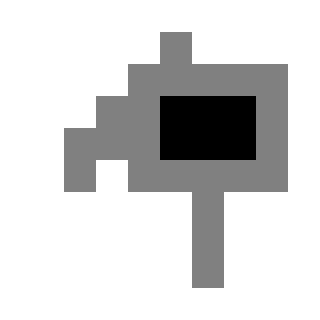
\includegraphics[width=0.40\textwidth]{mod3/figures/morphology-erosion.png}
	\caption{Erosion. Gray pixels indicate the original image. Black pixels remain after erosion with a 3x3 square. For display reasons, black pixels indicate foreground, white pixels background.}
	\label{fig:morphology-erosion}
\end{figure}

\minisec{Dilation}
In contrast to erosion, dilation grows or thickens an object in a binary image. A background pixel is changed to foreground if at least one pixel in the neighborhood is a foreground pixel (Fig. \ref{fig:morphology-dilation}). 

\begin{figure}[!ht]
	\centering
		
\includegraphics[width=0.40\textwidth]{mod3/figures/morphology-dilation.png}
	\caption{Dilation. Gray pixels indicate the dilated object. Black pixels are the original object.}
	\label{fig:morphology-dilation}
\end{figure}

\minisec{Opening and Closing}
The combination of dilation and erosion can be very useful to remove artefacts that remain in an image after thresholding. \emph{Opening} is an erosion followed by a dilation and used to smooth objects, break thin connections and remove protrusions. \emph{Closing} is a dilation followed by an erosion and used to smooth objects, join closely neighbored objects and fill small holes. 

\begin{taskbox}{Morphological operations}
\begin{enumerate}
	\item Open the image thresholded-nuclei.tif in /mod3/data. This image shows real thresholded nuclei with artificially introduced thresholding errors. 
	\item Perform erosion, dilation, opening and closing in \texttt{[Process > Binary]} and observe the changes of individual nuclei. Make sure you understand where the different operations enhance the image and where they make analysis more difficult.
	\item Instead of using opening or closing, try to manually erode 4-5 times and then dilate 4-5 times again; perform the same operations reversed. 
	\item Try the command \texttt{[Process > Binary > Fill Holes]}. This operation finds background areas that are completely surrounded by foreground and sets all those pixels to foreground.
	\end{enumerate}
\end{taskbox}

\subsection{Skeleton Analysis}
A skeleton analysis can be very useful if you are interested in the branching of a structure (neuronal arborizations, mitochondrial network, ..). Basically, your object becomes thinned (eroded) until only a single (center)line remains to describe the objects structure. 

\begin{taskbox}{Skeleton analysis}
\begin{enumerate}
	\item Open the image drosophila-ddac-neuron.tif in /mod3/data. In this task, you are going to analyze the arborization pattern of this, already thresholded, neuron. 
	\item Duplicate the image, do \texttt{[Plugins > Skeleton > Skeletonize]}. Make sure that the skeleton is white against a black background (you might need to invert the image). Now, edit the LUT so that the white pixels appear yellow, magenta or any other light color.
	\item Look at the original thresholded image and add the skeletonized image as an overlay (with zero transparent). Analyze the skeletonization results with the overlay.
	\item Perform \texttt{[Plugins > Skeleton > Analyze Skeleton]} on the skeletonized image. The Analyze Skeleton window allows you to prune the skeleton before analysis to get rid of small branches either by their length or intensity. Tick 'Show detailed info' and click on 'OK' (Fig. \ref{fig:analyze-skeleton-dialog}).
	
	\begin{minipage}[t]{\linewidth}
		\begin{center}
		\adjustbox{valign=t}{%
			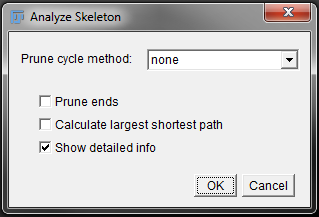
\includegraphics[width=0.4\textwidth]{mod3/figures/analyze-skeleton-dialog.png}%
		}
		\medskip
		\captionof{figure}{Analyze skeleton window.}\label{fig:analyze-skeleton-dialog}
		\end{center}
	\end{minipage}
	
	\item Three windows show up: Detailed information about each branch, summary results with branch statistics, and an image showing the skeleton with branch points and end points in different colors. You can try out different prune methods and compare the results. 
	
	\end{enumerate}
\end{taskbox}

\subsection{Watershed transform}
Watershed segmentation is used to separate touching objects, i.e. they appear as a single object in the binary image. The algorithm first calculates an Euclidean distance map (Fig. \ref{fig:distance-transform}), where the distance of each pixel to the nearest foreground pixel is calculated. The remaining black objects (peaks after the distance transform, centers of the original binary objects) are then dilated until the edge of the original object is found or the edge touches a region of another dilating object. This approach works best if the objects are 'round-ish' and have small overlap.

\begin{figure}[ht]
	\centering
		\includegraphics[width=0.60\textwidth]{mod3/figures/distance-transform.png}
	\caption{Distance transform}
	\label{fig:distance-transform}
\end{figure}

\begin{taskbox}{Watershed transform}
\begin{enumerate}
	\item Open the image bunch-of-nuclei.tif in /data/chapter4. Use the gauss-filter and thresholding to generate a binary image with the nuclei detected. Duplicate. 
	\item Use \texttt{[Process > Binary > Watershed]} on the binary image. Observe where the algorithm splits objects.
	\end{enumerate}
\end{taskbox}

\section{Analyzing objects}

Fiji has a very powerful method to obtain measurements from segmented objects which is called 'Analyze Particles' (Fig. \ref{fig:analyze-particles-dialog}). The windows allows you to select detected objects by size and by circularity, excluding objects at the edges of the image and produces several result outputs. It can add detected objects as individual ROIs to the ROI manager and perform calculations by performing the 'Measure' method on each detected object.

\begin{figure}[!ht]
	\centering
		\includegraphics[width=0.40\textwidth]{mod3/figures/analyze-particles-dialog.png}
	\caption{Analyze Particles Window}
	\label{fig:analyze-particles-dialog}
\end{figure}

\begin{taskbox}{Analyze Particles}
\begin{enumerate}
	\item Open the image bunch-of-nuclei.tif in /mod3/data and use a sequence of filtering, thresholding and binary operations to identify the nuclei. Remember that this image does not provide an easy perfect result on purpose!
	\item Set the measurements you want to perform \texttt{[Analyze > Set Measurements...]}. For this example, we want at least measure the area and the mean gray value. 
	\item Perform \texttt{[Analyze > Analyze Particles...]}. Do not select objects by size or circularity, show the outlines and tick 'Display results', 'Clear results', 'Add to Manager' and 'Summarize'.
	\item Several windows should show up. A summary report indicating the number of detected objects, and several average statistics; A results window showing the selected measurements for each detected object; an outline image indicating the object number for each object; the ROI Manager with each object as an individual ROI. Why is the mean intensity value $255$ for each object? The measurement was performed on the thresholded binary image. While thresholding does not change the shape of an object, the intensity values are obviously not maintained. In order to perform the measurements on the original image, Redirect the measurements to the original image in 'Set Measurements...'.
	\item Explore the functions of the particle-analyzer method and try to select objects in a way that only small/large or round objects are measured.
	\end{enumerate}
\end{taskbox}

\subsection{Working with Plugins: Trainable Segmentation}
Machine learning methods can be used to let the computer learn what you think as object and background. Fiji has a Trainable Weka Segmentation plugin. Using this plugin, you can manually mark pixels as signal or background and let the plugin 'learn' the differences between these two classes of pixels. To achieve this differences learning, the plugin uses many features of the pixels to come up with a model that categorizes the pixels into classes. 

\begin{taskbox}{Trainable Weka Segmentation}
\begin{enumerate}
	\item Open the image tissue-adipocytes.tif in /mod3/data if it is not already open.
	\item Go to \texttt{[Plugins > Segmentation > Trainable Weka Segmentation]}. A window pops up that shows the image and several buttons (Fig. \ref{fig:weka-segmentation-window}).
	
	\begin{minipage}[t]{\linewidth}
		\begin{center}
		\adjustbox{valign=t}{%
			\includegraphics[width=0.8\textwidth]{mod3/figures/weka-segmentation-window.png}%
		}
		\medskip
		\captionof{figure}{Trainable segmentation window.}\label{fig:weka-segmentation-window}
		\end{center}
	\end{minipage}
	
	\item Use the freehand line tool and draw on an image object you want to detect. Add this selection to class 1. Repeat this step and then add two background selections to class 2. 
	\item Click on 'Train classifier'. You should now see what the method thinks is background and foreground. If you click on 'Create result' a two color image is generated that can easily be converted into a binary image.
	
\end{enumerate}

You have now seen the most basic usage of this plugin. For example, you could use more than two classes or apply a learned classifier to more than one file.
\end{taskbox}


\bibliographystyle{plainnat}
\bibliography{coursebib}


\end{document}





